\documentclass[a4paper,article,14pt]{extarticle}

% Подключаем главный пакет со всем необходимым
\usepackage{spbudiploma}

% Пакеты по желанию (самые распространенные)
% Хитрые мат. символы
\usepackage{euscript}
% Таблицы
\usepackage{longtable}
\usepackage{makecell}
% Картинки (можно вставлять даже pdf)
\usepackage[pdftex]{graphicx}

\usepackage{amsthm,amssymb, amsmath}
\usepackage{textcomp}

\usepackage{minted} % для примеров кода (требует параметра -shell-escape)
\usemintedstyle{bw}


\begin{document}

% Титульник в файле titlepage.tex
\newgeometry{left=30mm, top=20mm, right=15mm, bottom=20mm, nohead, nofoot}
\begin{titlepage}
\begin{center}

\textbf{Санкт--Петербургский государственный университет}\\
\textbf{Факультет математики и компьютерных наук}


\vspace{35mm}

\textbf{\textit{\large Добрынин Иван Ильич}} \\[8mm]
% Название
\textbf{\large Выпускная квалификационная работа}\\[3mm]
\textbf{\textit{\large Разработка комплекса информационных систем для проведения соревнований и тренировок по спортивному~программированию в формате дуэли}}

\vspace{20mm}
Уровень образования: бакалавриат\\
Направление 01.03.02 «Прикладная математика и информатика»\\
Основная образовательная программа СВ.5156.2022
«Современное программирование»\\[25mm]


% Научный руководитель, рецензент
\begin{flushright}
\begin{minipage}[t]{0.65\textwidth}
{Научный руководитель:} \\
к.ф.-м.н. Д.\,С.\,Шалымов
\vspace{10mm}

{Рецензент:} \\
к.ф.-м.н. В.\,А.\,Голодов
\end{minipage}
\end{flushright}

\vfill

{Санкт-Петербург}
\par{\the\year{} г.}
\end{center}
\end{titlepage}
\restoregeometry
\addtocounter{page}{1}

% Содержание
\tableofcontents
\pagebreak

\specialsection{Введение}

Спортивное программирование в наше время приобретает всё большую популярность.
Проводятся всероссийские и международные соревнования.
В них участники решают алгоритмические задачи, которые требуют от них не только теоретических знаний,
но и практических навыков программирования, среди которых важную роль играет умение быстро и эффективно писать код.

Общепринятым форматом проведения соревнований является контест, индивидуальный или командный,
в котором может быть любое количество участников.
Зачастую контест содержит набор задач разной сложности, на решение которых отводится вплоть до пяти часов времени.
Участники соревнуются в количестве решённых задач либо в суммарном количестве баллов, набранных за решения задач.

Стандартная задача по спортивному программированию обычно состоит из условия, описания формата входных и выходных данных,
ограничений по времени и памяти, а также набора тестов.
Для решения задачи требуется написать код на одном из разрешённых языков программирования,
который будет обрабатывать входные данные и выдавать результат в соответствии с условием задачи.
В условии, как правило, приводятся открытые примеры тестов с правильными ответами,
а полная и окончательная проверка решения выполняется на скрытых тестах, недоступных участнику во время соревнования.

Формат дуэли представляет собой соревнование между двумя участниками,
которые одновременно решают одну и ту же задачу и стараются сделать это быстрее друг друга.
Такой вид соревнования вызывает больший интерес и повышает вовлечённость участников,
так как они соревнуются не с абстрактным списком соперников, а с одним конкретным человеком.
Дуэль обычно представляет собой короткое соревнование с более простыми задачами,
что требует высокой концентрации и быстроты действий в течение меньшего промежутка времени.
Участники отрабатывают и проявляют навыки эффективного написания кода,
а также умение находить и исправлять ошибки в условиях стресса и ограниченного времени, чтобы решить задачу раньше соперника.

Существующие платформы для спортивного программирования в основном ориентированы на проведение контестов
и не предоставляют достаточной гибкости и возможности для организации дуэлей по пользовательским правилам.
Дополнительный интерес вызывает анализ поведения участников в дуэлях и выявление закономерностей,
которые могут быть использованы для выявления нечестных пользователей,
использующих сторонние инструменты для получения преимущества.
Особенно актуальной становится задача отслеживания несанкционированного применения инструментов искусственного интеллекта,
способных генерировать готовые фрагменты решений или полностью решать задачу за участника.
Оперативное выявление таких случаев необходимо для сохранения духа честного соревнования,
в котором результат определяется навыками, подготовкой и скоростью самого участника.

В связи с этим возникает необходимость в разработке платформы для проведения дуэлей по спортивному программированию,
поддерживающей различные форматы дуэлей и турниров, автоматическое тестирование решений участников,
а также сбор и анализ информации о поведении участников для выявления возможных нарушений правил.


\specialsection{Постановка задачи}

\begin{itemize}
\item Определить функциональные и нефункциональные требования к разрабатываемому комплексу информационных систем.
\item Спроектировать масштабируемую и отказоустойчивую архитектуру платформы.
\item Реализовать систему проведения дуэлей и взаимодействия с пользователями.
\item Реализовать систему автоматического тестирования решений участников.
\item Реализовать систему анализа поведения участников и выявления возможных нарушений правил.
\item Провести тестирование разработанной платформы и оценку работы реализованных компонентов.
\end{itemize}


\section{Обзорный раздел по предметной области}

Существуют различные платформы для решения задач по спортивному программированию, например Codeforces, LeetCode, CodeBattle.
Однако они не всегда предоставляют требуемые возможности.
Сравнительный анализ этих платформ представлен в таблице \ref{platforms-comparison}.

Возможность вызвать конкретного соперника на дружескую дуэль широко распространена в
соревновательных платформах других предметных областей, например в онлайн-шахматах.
Для спортивного программирования такой сценарий также естественен, однако существующие платформы чаще
ориентированы на контесты и не рассматривают дуэли основным режимом взаимодействия участников.

Единственной из рассматриваемых платформ, которая поддерживает формат дуэлей, является CodeBattle.
Однако она не предоставляет достаточной гибкости для организации пользовательских форматов соревнований.
В отличие от других платформ, CodeBattle не предоставляет возможности проведения турниров с собственным набором задач.
Нестандартные типы задач, которые отличаются от общепринятых в спортивном программировании, не поддерживаются ни одной из платформ.

Ни одна из платформ также не предоставляет возможности анализа поведения участников во время написания кода и участия в дуэли,
что ограничивает возможности контроля честности соревнований.

\begin{table}[ht]
\begin{center}
\begin{tabular}{lccc}
     & 
\includegraphics[height=0.6cm]{images/codeforces-logo.png} & 
\includegraphics[height=0.6cm]{images/leetcode-logo.png} & 
\includegraphics[height=0.6cm]{images/codebattle-logo.png} \\
\hline
    Поддержка формата дуэлей & $-$ & $-$ & $+$ \\
    Настройка правил соревнований & $-$ & $-$ & $\pm$ \\
    Использование своих задач & $+$ & $\pm$ & $-$ \\
    Нестандартные типы задач & $-$ & $-$ & $-$ \\
    Анализ поведения участников & $-$ & $-$ & $-$ \\
\end{tabular}
\caption{
\label{platforms-comparison}
     Сравнение платформ.}
\end{center}
\end{table}

Также стоит отметить, что для проведения соревнования задача предварительно подготавливается автором в виде пакета,
который содержит условие, тесты, ограничения, эталонное решение, а при необходимости генераторы тестов,
валидаторы входных данных и чекер для проверки ответа.
Одним из распространённых инструментов для подготовки таких пакетов является Polygon,
формат которого используется на многих соревнованиях по спортивному программированию.

Таким образом, существующие платформы не обеспечивают одновременно поддержку настраиваемых дуэлей, проведения турниров,
расширяемых форматов задач и анализа поведения участников.
Это определяет необходимость разработки собственного комплекса информационных систем, который будет удовлетворять этим требованиям.


\section{Требования к системе}

На основе проведённого анализа существующих платформ были сформулированы требования к
разрабатываемому комплексу информационных систем.
Требования разделены на функциональные и нефункциональные.

\subsection{Функциональные требования}

\subsubsection*{Пользователи}
Система должна обеспечивать регистрацию и аутентификацию пользователей по никнейму и паролю.
Пользователь идентифицируется по уникальному никнейму.

\subsubsection*{Группы пользователей}
Система должна поддерживать создание и управление группами пользователей.
Группа идентифицируется по уникальному числовому идентификатору.
Пользователи в группе могут иметь роли создателя, менеджера и участника,
которые определяют их права на совершение действий в группе.
Пользователи могут быть добавлены в группу с определённой ролью, которая впоследствии может быть изменена.
Пользователи с более высокими правами могут исключать пользователей с меньшими правами из группы,
а также покинуть группу самостоятельно.

\subsubsection*{Рейтинг пользователя}
Система должна реализовывать рейтинговую систему.
Пользователь получает начальный рейтинг при регистрации.
Рейтинг меняется при участии пользователя в рейтинговых дуэлях.

\subsubsection*{Рейтинговая дуэль}
Система должна поддерживать рейтинговый режим дуэли.
Пользователь может начать поиск рейтинговой дуэли,
и система должна подобрать соперника, близкого по рейтингу.
Рейтинг меняется в соответствии с результатом дуэли и текущими рейтингами участников.

\subsubsection*{Дружеская дуэль}
Система должна поддерживать дружеский режим дуэли.
Пользователь может отправить приглашение на дружескую дуэль другому пользователю.
Второй пользователь имеет возможность принять и отклонить приглашение.
Рейтинг после дружеской дуэли не меняется.

\subsubsection*{Конфигурация дуэли}
Система должна поддерживать управление конфигурацией дуэли.
Пользователь может создать и отредактировать конфигурацию дуэли.
В конфигурацию дуэли входят следующие параметры:
\begin{itemize}
\item длительность дуэли;
\item возможность смотреть код соперника во время дуэли;
\item количество задач в дуэли;
\item этапность задач в дуэли (все задачи доступны сразу или открываются по очереди);
\item сложность и темы каждой задачи в дуэли.
\end{itemize}
Имеется стандартная конфигурация дуэли, по которой проводятся рейтинговые дуэли.
Пользователь имеет возможность использовать для дружеской дуэли любую из своих конфигураций.

\subsubsection*{Дуэль в группе}
Система должна предоставлять возможность создания дуэли в группе между определёнными пользователями.
Пользователи с определёнными ролями имеют возможность создать дуэль со своей конфигурацией между любыми двумя участниками группы.
Дуэль в таком случае является нерейтинговой.

\subsubsection*{Турнир в группе}
Система должна предоставлять возможность создания турнира в группе.
Турнир имеет схему проведения (например, олимпийская система или групповая стадия).
Для всех дуэлей в турнире можно выбрать единую конфигурацию дуэли.
Можно выбрать пользователей группы, которые будут участвовать в турнире.

\subsubsection*{Участие в дуэли}
Интерфейс участия в дуэли поделён на две части.
В одной отображается редактор кода, в котором пользователь должен писать своё решение задачи.
Во второй отображается условие задачи и наборы открытых тестовых данных.
Участник дуэли имеет возможность отправить текущее решение на проверку и получить вердикт тестирования.
В дуэли побеждает пользователь, который раньше другого отправит первое правильное решение.
Если по истечении длительности дуэли правильных решений отправлено не было, объявляется ничья.

\subsubsection*{Запуск решения на тестах}
Интерфейс участия в дуэли предоставляет возможность запустить своё решение на открытых тестах и увидеть выходные данные.
Также пользователь имеет возможность запустить своё решение на своём произвольном тесте.

\subsubsection*{Автоматическое тестирование решений}
Система должна автоматически тестировать решения пользователей.
Это подразумевает компиляцию и/или запуск пользовательского кода с последующей проверкой правильности ответа.
Система должна поддерживать выполнение решений на нескольких языках программирования.
Проверка корректности ответа может осуществляться с использованием специальной программы --- чекера.
Каждая задача имеет ограничение по времени и по памяти для выполнения решения,
и система должна корректно обрабатывать случаи превышения времени выполнения или используемой памяти во время выполнения.

\subsubsection*{История дуэлей}
Система должна предоставлять возможность просмотра истории прошедших дуэлей.
Пользователь должен иметь возможность просматривать посылки, сделанные во время участия в дуэли,
а также отправлять решения на проверку после завершения дуэли.

\subsubsection*{Анализ поведения участников}
Система должна собирать информацию о действиях пользователя во время участия в дуэли,
включая события редактирования кода и отправки решений.
На основе собранной информации система должна иметь возможность анализировать поведение участников
и определять степень подозрительности пользователя в конкретной дуэли.

\subsection{Нефункциональные требования}

\subsubsection*{Производительность}

Система должна поддерживать одновременное тестирование нескольких решений.
Результаты тестирования должны отображаться пользователю с минимальной задержкой.

\subsubsection*{Масштабируемость}

Архитектура системы должна поддерживать горизонтальное масштабирование отдельных компонентов при росте нагрузки.

\subsubsection*{Отказоустойчивость}

Система должна быть устойчива к отказу отдельных внутренних и инфраструктурных компонентов.
Система должна обеспечивать возможность восстановления работы после сбоев отдельных компонентов.

\subsubsection*{Безопасность}

Система должна обеспечивать безопасное выполнение пользовательского кода в изолированной среде без доступа к ресурсам хостовой системы.

\subsubsection*{Расширяемость}

Архитектура системы должна поддерживать добавление новых форматов задач без значительного изменения существующих компонентов.
Система должна поддерживать расширение правил проведения дуэлей и турниров.

\subsubsection*{Наблюдаемость}

Система должна поддерживать сбор метрик, журналирование событий и мониторинг состояния компонентов,
а также предоставлять необходимые данные для выявления сбоев.

\subsubsection*{Модульность}

Компоненты системы должны быть слабо связаны между собой и поддерживать независимое развёртывание.

\section{Архитектура системы}

Для реализации требований была разработана распределённая микросервисная архитектура,
которая состоит из нескольких основных и инфраструктурных компонентов и представлена на рисунке \ref{architecture}.

\begin{figure}[ht]
\begin{center}
\scalebox{0.25}{
   
\includegraphics{images/architecture.png}
}
\caption{
\label{architecture}
     Архитектура системы.}
\end{center}
\end{figure}

\subsection{Интерфейс взаимодействия с пользователем}

Компонент представляет собой web-приложение, разработанное с использованием React JS.
Он обеспечивает взаимодействие пользователя с системой.

Использование web-приложения позволяет обеспечить кроссплатформенность системы, так как для работы требует наличие любого браузера.
Взаимодействие Frontend-приложения с Backend-компонентами осуществляется по HTTP и WebSocket через nginx.
Nginx используется в качестве обратного прокси и балансировщика нагрузки.

В качестве подхода к структурной схеме приложения был выбран Feature Sliced Design (FSD).
Он предполагает разделение кода на независимые и переиспользуемые модули и слои,
что упрощает сопровождение и развитие системы при появлении новых функциональных требований.
Структура веб-приложения представлена на рисунке \ref{frontend-structure}.

\begin{figure}[ht]
\begin{center}
\scalebox{0.2}{
   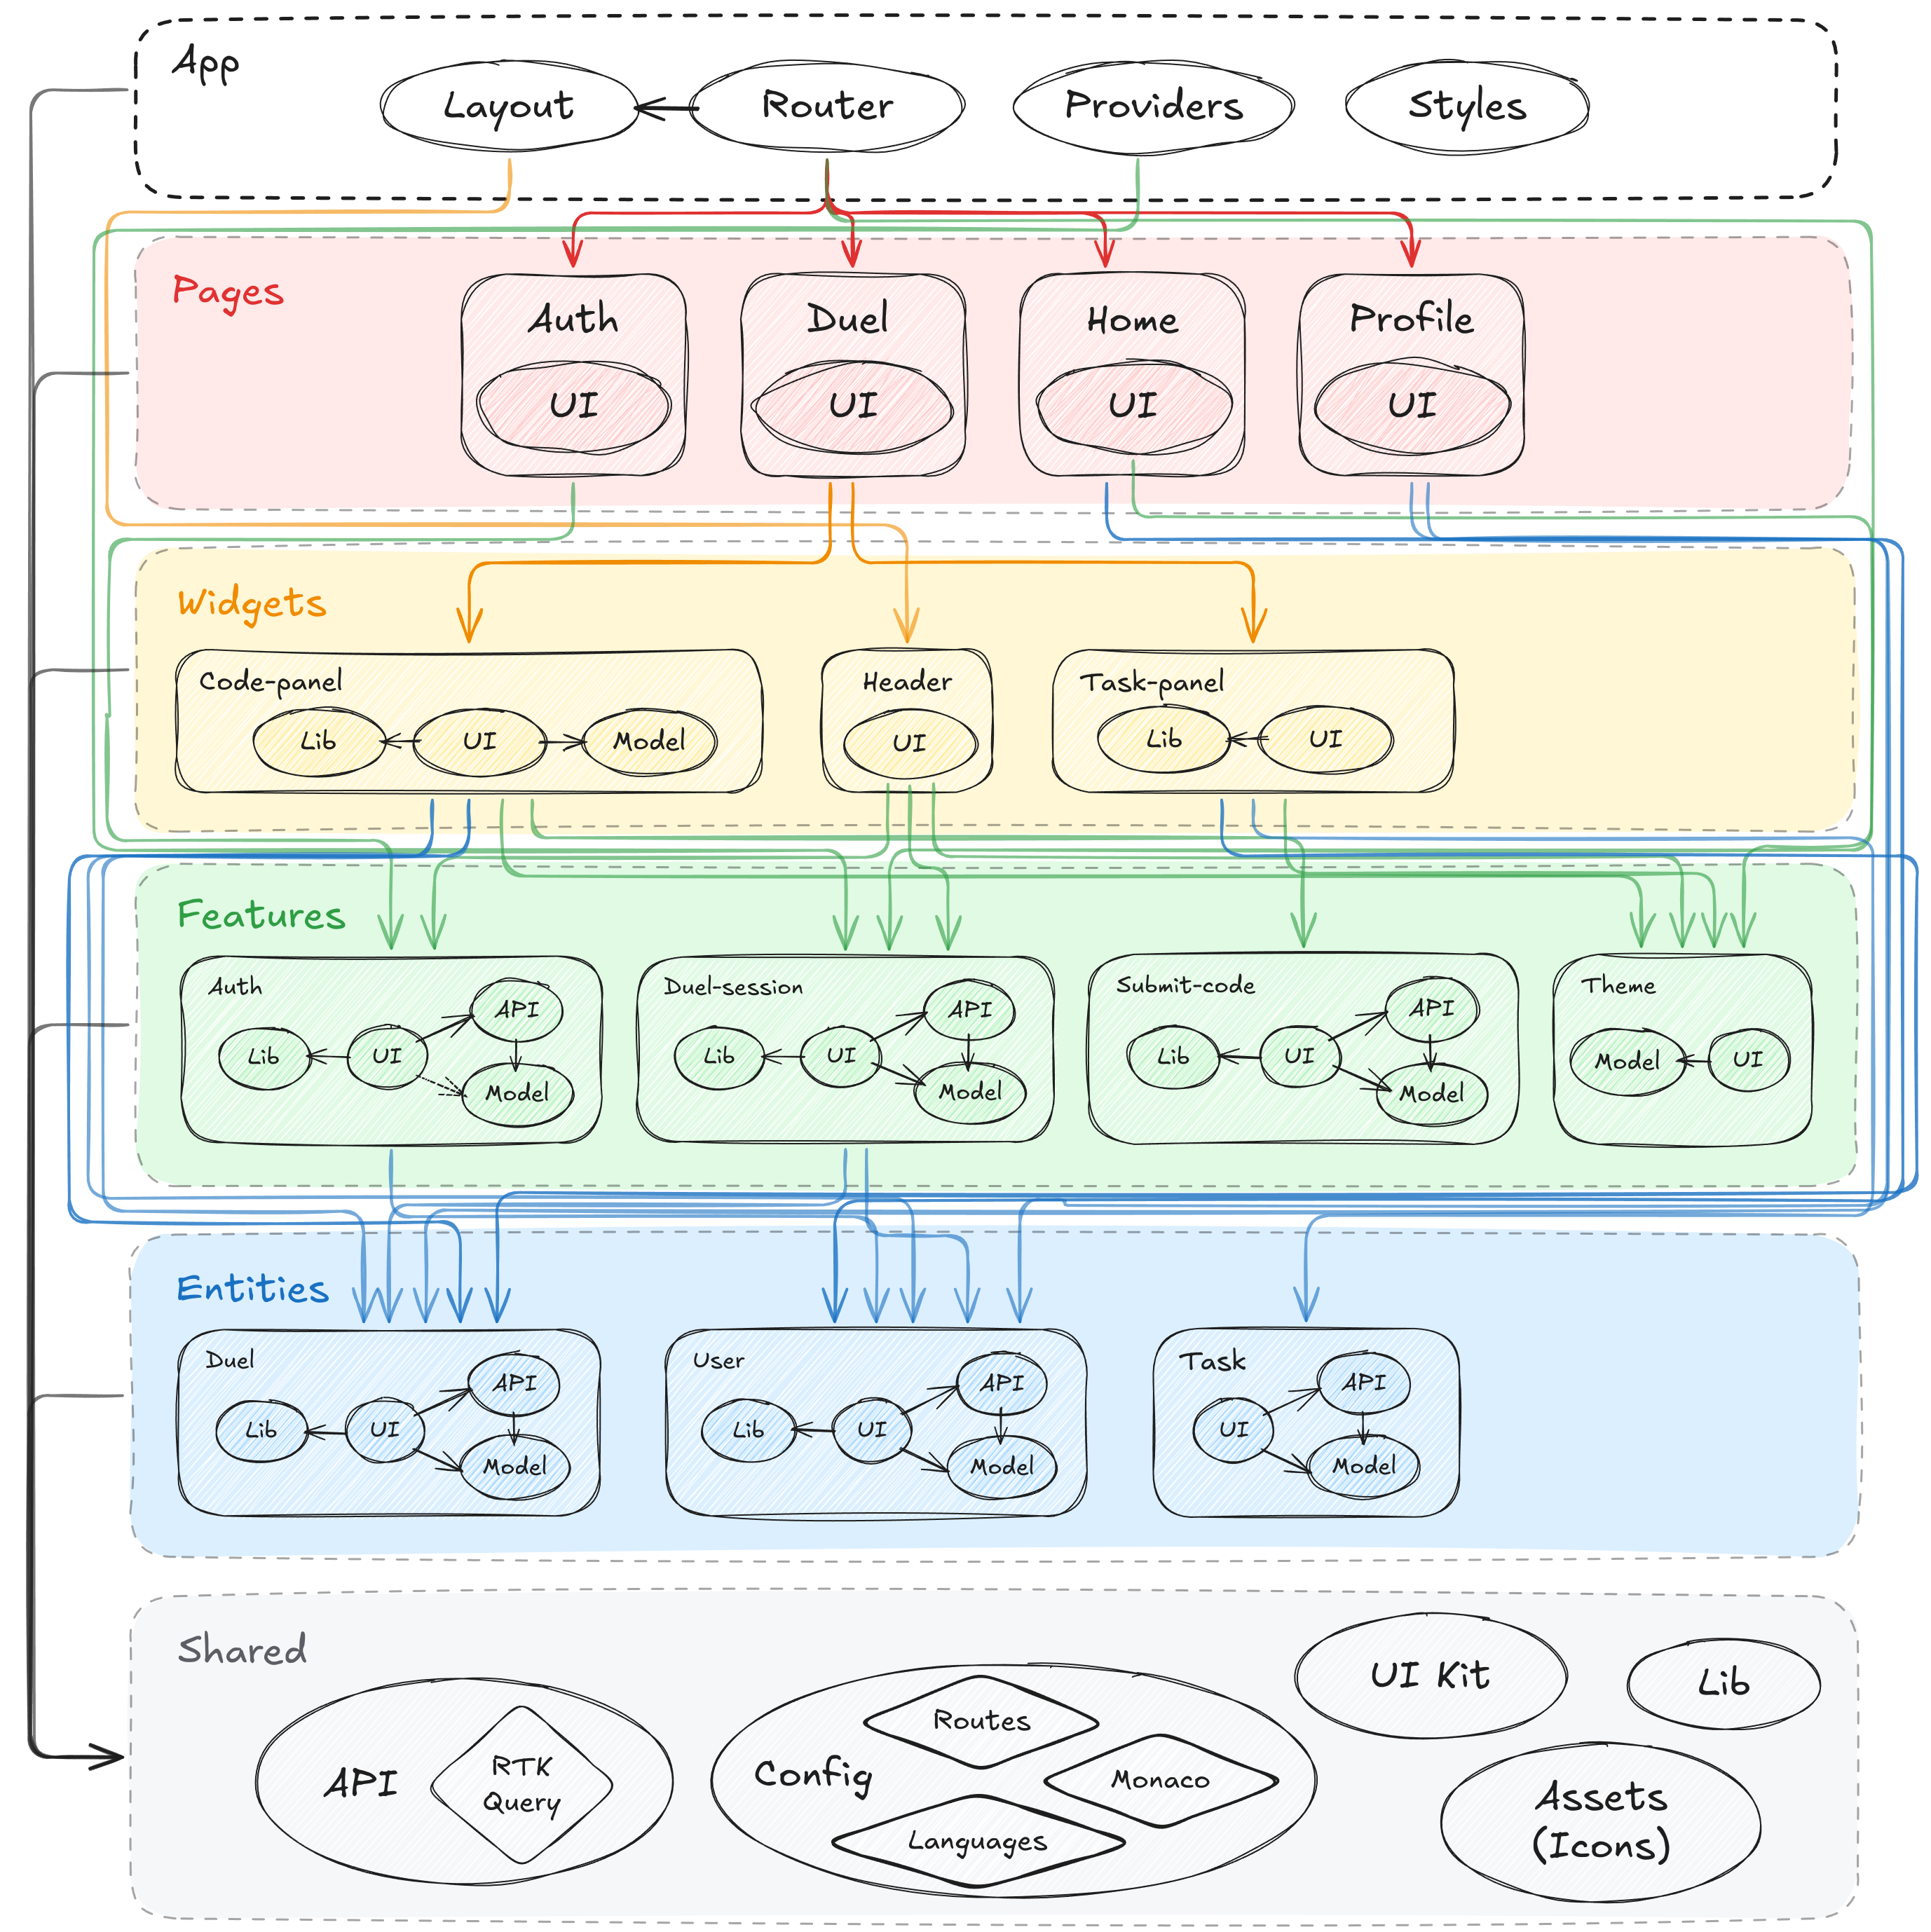
\includegraphics{images/frontend-structure.png}
}
\caption{
\label{frontend-structure}
     Структура веб-приложения.}
\end{center}
\end{figure}

В качестве редактора кода в web-интерфейсе используется библиотека Monaco Editor.
Редактор схож с VS Code и поддерживает подсветку синтаксиса, работу с несколькими языками программирования,
а также предоставляет возможность сбора списка действий пользователя во время написания кода.

Приложение поддерживает выбор светлой и тёмной темы интерфейса, что позволяет повысить удобство использования системы
при различных условиях освещения и длительной работы с платформой.

\subsection{Компонент управления пользователями и дуэлями}

Компонент Duely представляет собой приложение на C\# с использованием ASP.NET,
в котором реализуется логика взаимодействия с пользователями,
а также бизнес-логика, относящаяся к управлению группами, проведению дуэлей и турниров.
Кроме того компонент отвечает за приём решений пользователей и их передачу в подсистему автоматического тестирования.

Подход к структуре приложения сочетает в себе подходы из чистой и гексагональной архитектуры.
Код приложения разбит на .NET-проекты (модули) с целью фиксации направлений зависимостей компонентов друг от друга.
Структура приложения Duely представлена на рисунке \ref{duely-structure}.

\begin{figure}[ht]
\begin{center}
\scalebox{0.2}{
   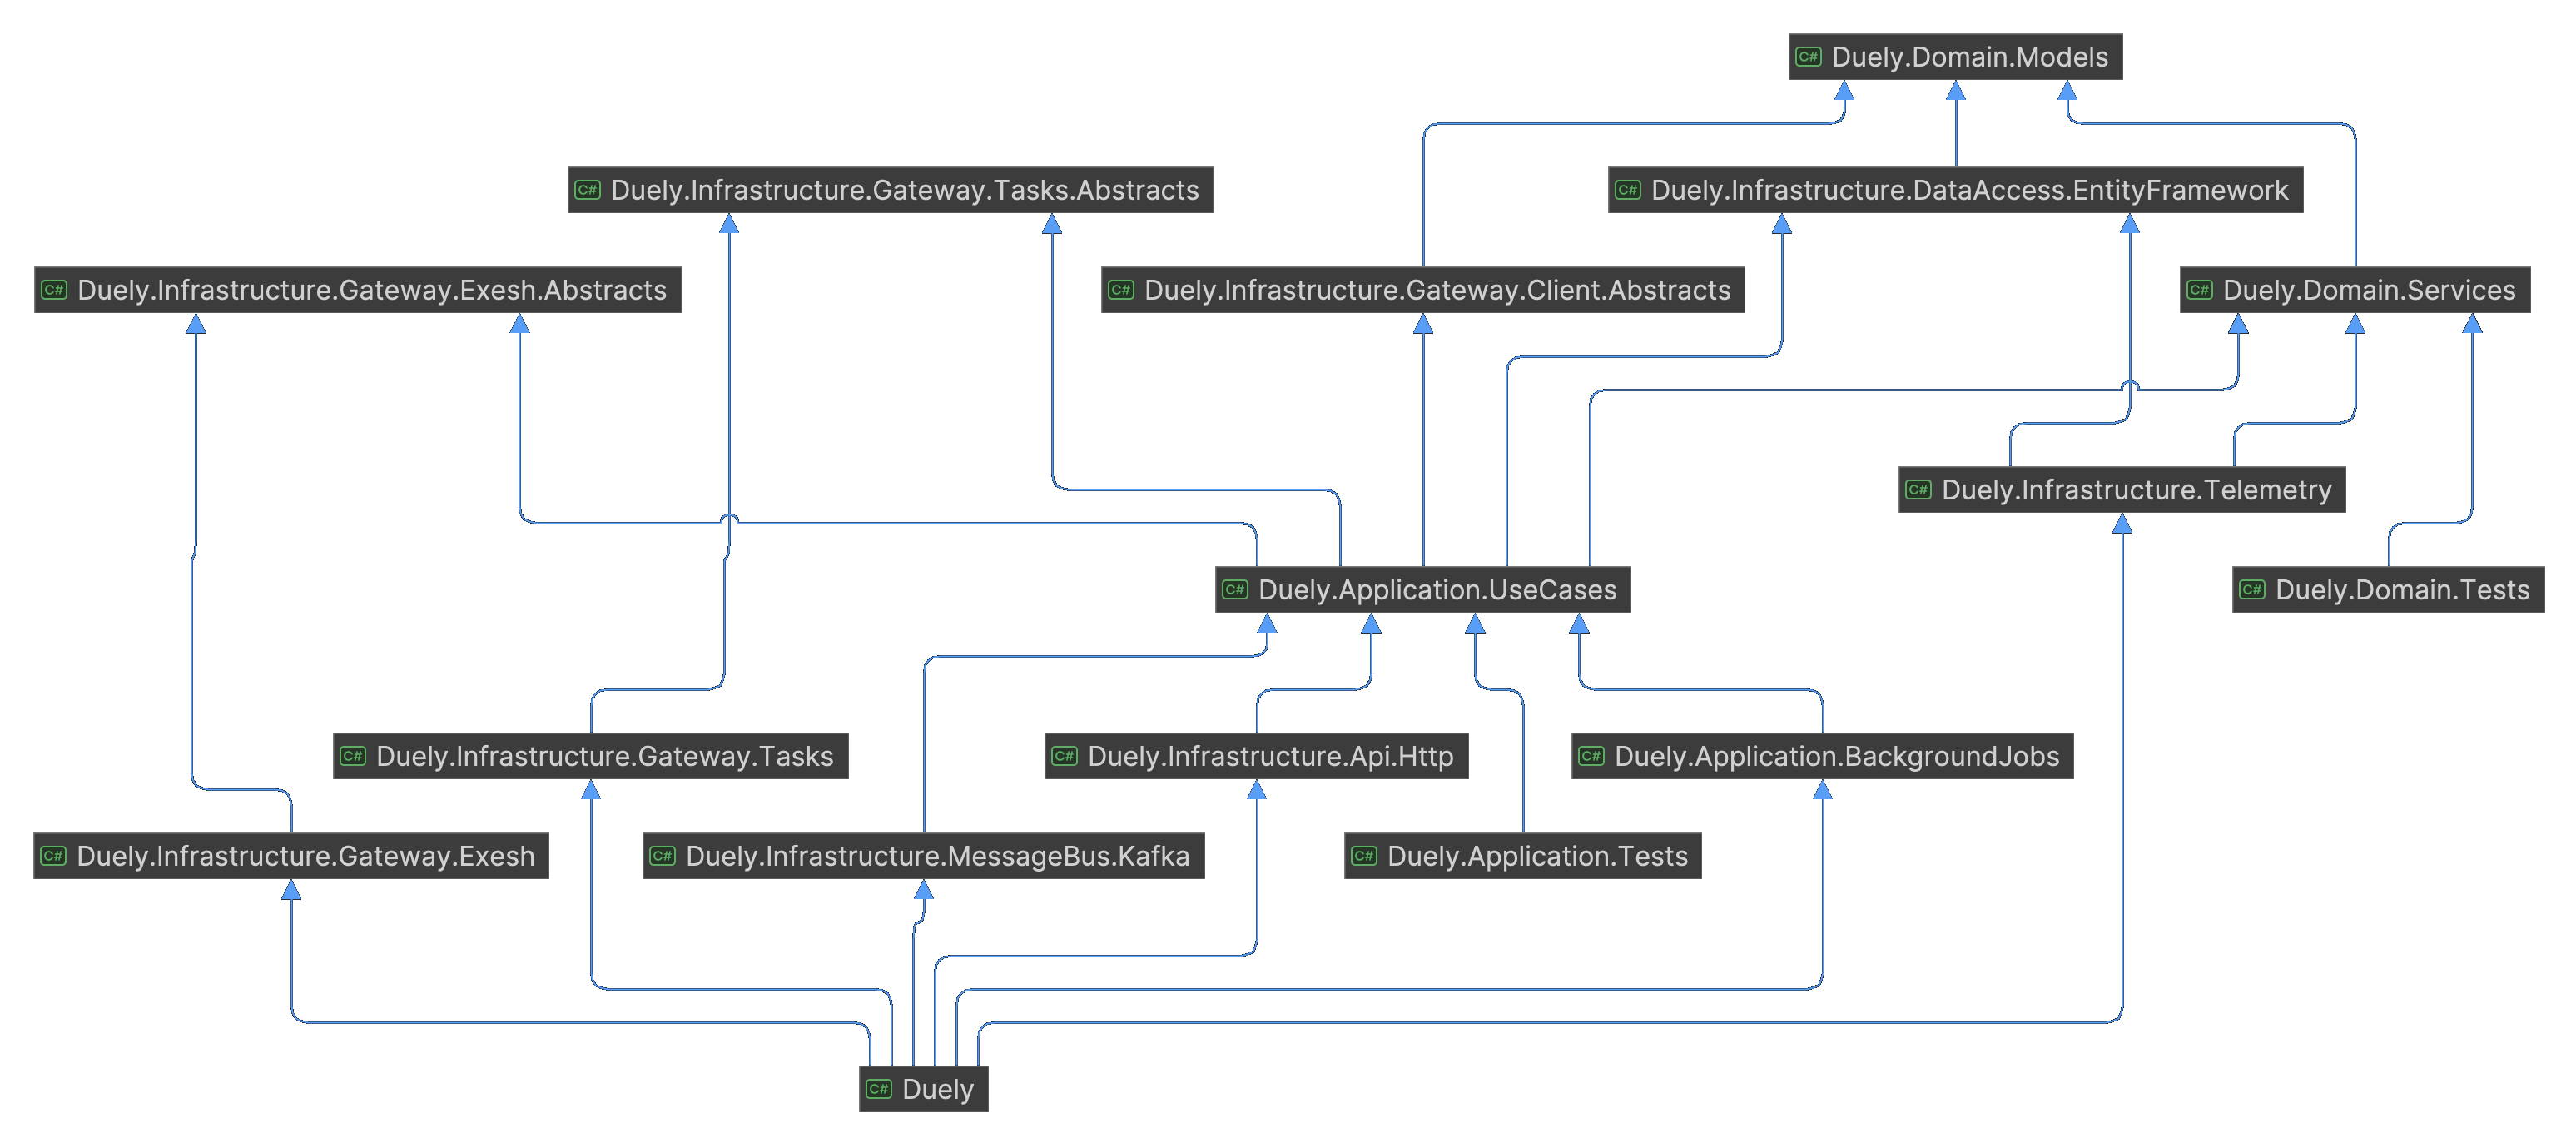
\includegraphics{images/duely-structure.png}
}
\caption{
\label{duely-structure}
     Структура приложения Duely.}
\end{center}
\end{figure}

В качестве базы данных используется PostgreSQL.
Выбор был сделан, исходя из широких возможностей СУБД для работы с реляционными данными,
поддержкой транзакционности и относительной простотой эксплуатации.
Для работы с БД в коде приложения и миграции схемы данных используется Entity~Framework.

Для авторизации запросов используется JWT токен, который выписывается при аутентификации по никнейму и паролю пользователя.
При выписке access токена также выписывается refresh токен, который используется для обновления access токена при окончании действия.

Используется двунаправленное WebSocket соединение с Frontend,
по которому отправляются события изменения кода пользователя в редакторе, а также изменения статуса тестирования решения.
Для авторизации запроса на установление соединения используется одноразовый token,
который выписывается компонентом Duely и прикладывается приложением Frontend к запросу на WebSocket соединение.

Для реализации взаимодействия с другими компонентами, вызванного реакцией на произошедшее в системе событие,
используется паттерн транзакционный Outbox.
Вместе с обновлением данных доменных моделей в БД сохраняется запись в таблицу Outbox о том,
о необходимости выполнения некоторого отложенного действия (например, отправить сообщение определённому пользователю в WebSocket).
Запущенный фоновый процесс сканирует записи этой таблицы, выполняет диспетчеризацию и необходимую обработку.
Использование данного паттерна позволяет добиться гарантии обработки события At~Least~Once.

\subsection{Компонент анализа поведения пользователя}

Компонент Analyzer представляет собой приложение на Python, предназначенное для анализа действий пользователя во время дуэли.

При помощи библиотеки FastAPI реализовано API,
с помощью которого можно получить степень подозрительности пользователя по списку его действий во время дуэли.
Для анализа степени подозрительности с использованием библиотеки scikit-learn реализованы и обучены ML-модели.

\subsection{Компонент менеджмента задач}

Компонент Taski представляет собой приложение на Go и используется для хранения и управления задачами,
а также определяет правила автоматического тестирования решений и вердикты тестирования.

Выделение управления задачами в отдельный компонент позволяет независимо от других компонентов развивать и использовать компонент.
Структура доменного слоя позволяет расширять систему новыми типами задач и сценариями их тестирования
без необходимости существенного изменения других компонентов системы.

В компоненте реализован свой формат хранения метаданных о задаче, а также конвертер из общепринятого формата polygon во внутренний.
Все файлы, необходимые для тестирования задачи (тесты, решение, чекер), хранятся в файловой системе.
Взаимодействие с файловой системой выполняется при помощи библиотеки filestorage.

\subsection{Компонент запуска команд тестирования}

Компонент Exesh представляет собой приложение на Go и используется для запуска произвольных команд, необходимых для тестирования задач.

Внутренняя архитектура Exesh представлена на рисунке \ref{exesh-architecture}
и включает два вида компонентов, которые образуют модель оркестрации.
Центральным компонентом является coordinator.
В нём содержится API, а также вся логика управления исполнением команд.
За выполнение команд и сохранение артефактов запуска отвечает worker.

\begin{figure}[ht]
\begin{center}
\scalebox{0.4}{
   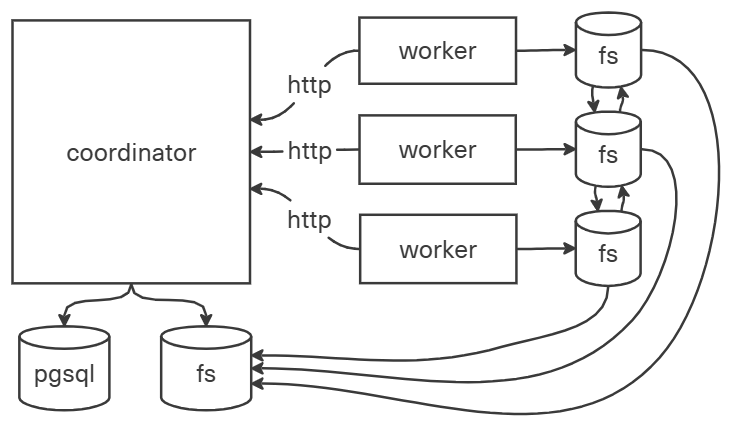
\includegraphics{images/exesh-architecture.png}
}
\caption{
\label{exesh-architecture}
     Архитектура компонентов внутри приложения Exesh.}
\end{center}
\end{figure}

Кластер представляет собой объединение одного coordinator и набора workers.
Горизонтальное масштабирование может быть достигнуто при помощи увеличения количества workers в кластере либо количества кластеров.
После запуска каждый worker регистрируется у заранее определённого coordinator,
а затем с некоторым интервалом выполняет запросы heartbeat для получения новых и передачи результатов выполненных команд.

Каждый coordinator и worker взаимодействует с локальным хранилищем при помощи библиотеки filestorage.
Результатом выполнения каждой команды является артефакт, который сохраняется в локальное хранилище.
Артефакты передаются между компонентами системы также при помощи библиотеки filestorage,
которая реализует передачу ресурсов в формате tar-stream с использованием сжатия.

\subsection{Компонент мониторинга работы системы}

Компонент Dashboard представляет собой приложение на Python с использованием библиотеки Django
и предназначен для визуализации работы Exesh в режиме реального времени.

Изначально для мониторинга планировалось использовать Grafana для сбора метрик и отрисовки дашбордов,
однако для графиков требуется высокая детализация временных событий,
так как за маленький промежуток времени может произойти много изменений.
Поэтому было принято решение реализовать своё приложение,
которое получает из БД все необходимые данные и формирует изображения с графиками.

\subsection{Взаимодействие компонентов}

Frontend и Duely имеют постоянное web-socket соединение,
с помощью которого достигается быстрота обновления интерфейса после каких-либо событий.
Все бэкенд-компоненты предоставляют REST API для взаимодействия с ними.
Для устранения циклических зависимостей и жёсткой связанности между компонентами,
а также для реализации асинхронного взаимодействия внутри некоторых процессов используется брокер обмена сообщениями.
В данном случае выбрана Kafka,
так как предоставляет средства горизонтального масштабирования и обеспечивает отказоустойчивую доставку сообщений.

\subsubsection*{Тестирование решений}

Тестирование решения инициируется пользователем на Frontend и задействует все основные компоненты системы.
Процесс представлен на рисунке \ref{testing-pipeline}.

\begin{figure}[ht]
\begin{center}
\scalebox{0.5}{
   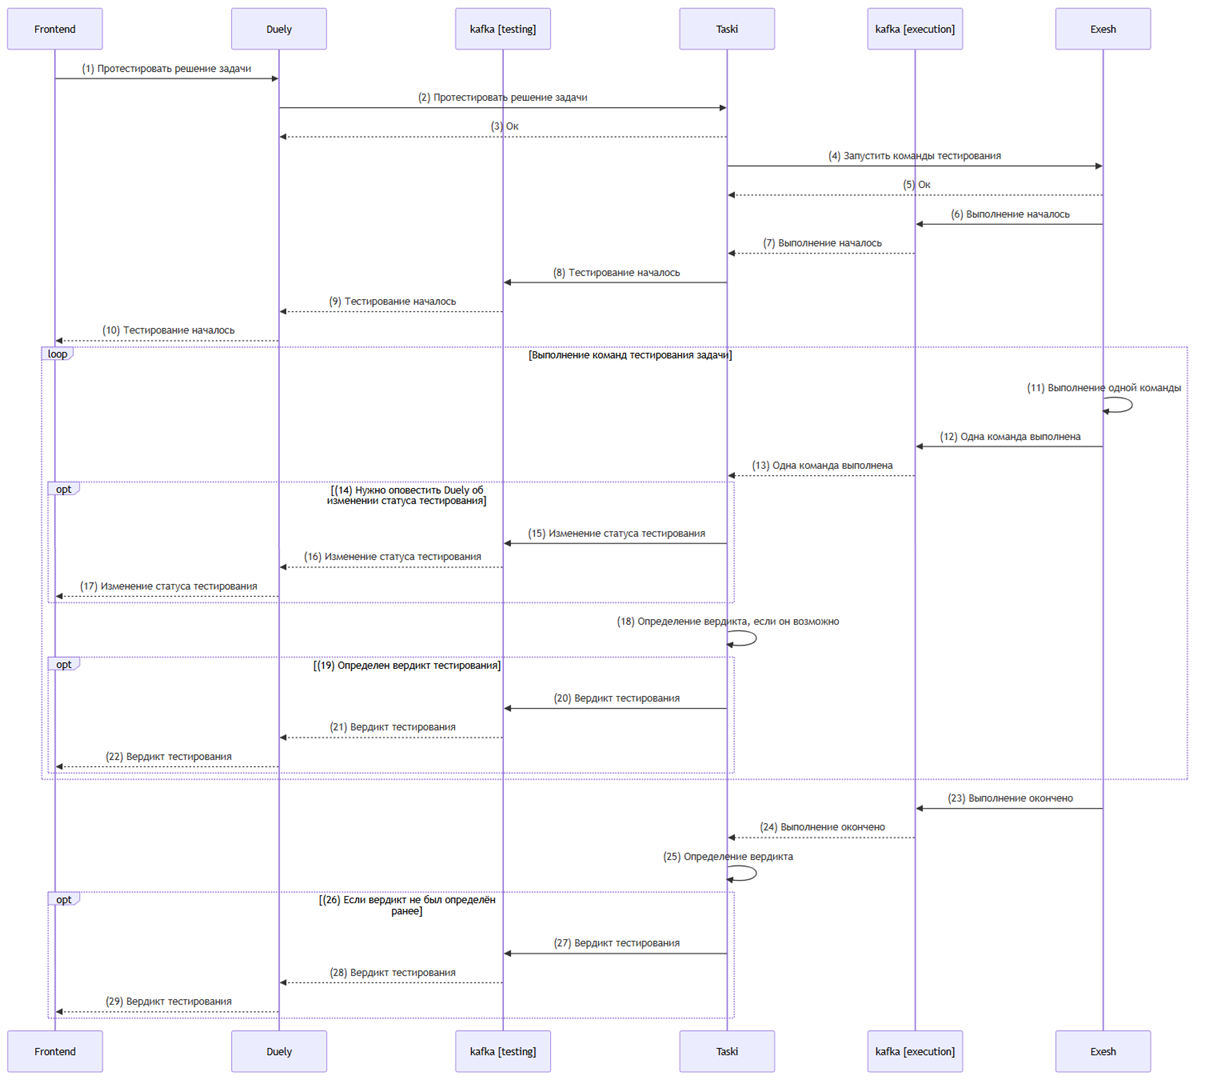
\includegraphics{images/testing-pipeline.png}
}
\caption{
\label{testing-pipeline}
     Процесс тестирования решения.}
\end{center}
\end{figure}

Frontend имеет web-socket соединение с Duely через nginx и отправляет обычный http запрос на тестирование решения задачи (1),
а далее ожидает сообщения с изменением статуса тестирования в web-socket соединение.
Duely выполняет http запрос в Taski на тестирование решения задачи (2)
и при успешном ответе (3) далее ожидает сообщения с изменением статуса тестирования в kafka из топика testing.
Taski делает http запрос в Exesh на запуск команд тестирования решения задачи (4)
и при успешном ответе (5) далее ожидает сообщения с результатами выполнения команд в kafka из топика execution.
Exesh при запуске команд отправляет сообщение о начале выполнения команд в kafka в топик execution (6).
Taski при получении сообщения о начале выполнения команд (7) отправляет сообщение о начале тестирования в kafka в топик testing (8).
Duely при получении сообщения о начале тестирования (9) отправляет сообщение
о начале тестирования в web-socket соединение с Frontend (10).
Exesh при выполнении каждой команды (11) отправляет событие о выполнении команды в kafka в топик execution (12).
Taski при получении сообщения о выполнении команды (13) отправляет сообщение
об изменении статуса тестирования в kafka в топик testing (15), если нужно оповестить Duely об этом (14).
Duely при получении сообщения об изменении статуса тестирования отправляет сообщение
об изменении статуса тестирования в web-socket соединение с Frontend (16).
Taski после получения каждого сообщения о выполнении команд (13) определяет вердикт тестирования (18),
если его можно определить (19), и отправляет его в kafka в топик testing (20).
Exesh при окончании выполнения команд отправляет сообщение о завершении выполнения команд в kafka в топик execution (23).
Taski при получении сообщения об окончании выполнения команд (24) определяет вердикт тестирования (25),
если он не был определен ранее (26), и отправляет его в kafka в топик testing (27).
Duely при получении сообщения с вердиктом (21, 28) тестирования отправляет его в web-socket соединение с Frontend (22, 29).

\subsubsection*{Выполнение кода на входных данных}

При написании кода пользователем в редакторе кода на странице платформы возникает потребность
запуска этого кода на произвольных входных данных с целью получить результат работы кода и отловить ошибки.
Выполнение кода не задействует компонент Taski, так как для него не требуются никакие данные о задаче.
Процесс представлен на рисунке \ref{run-code-pipeline}.

\begin{figure}[ht]
\begin{center}
\scalebox{0.8}{
   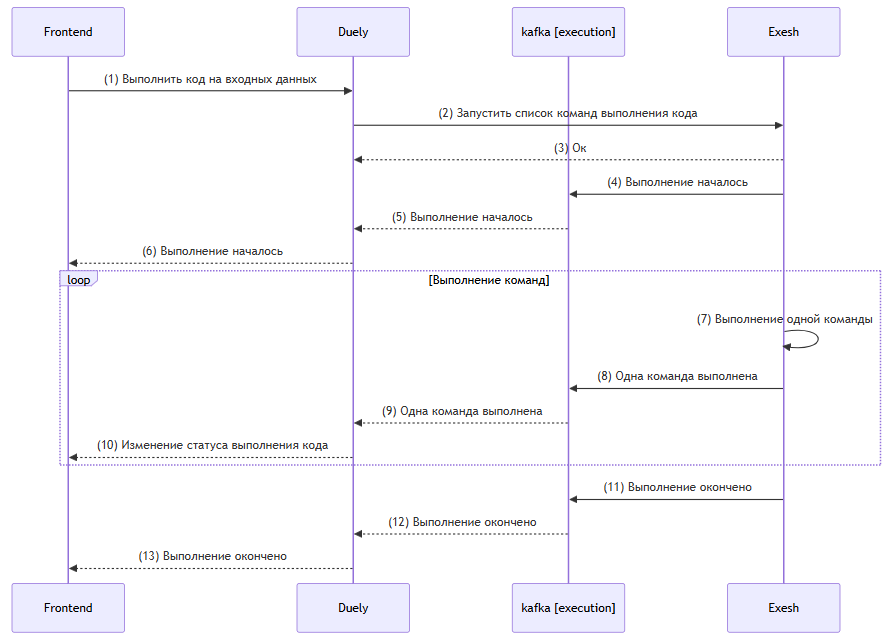
\includegraphics{images/run-code-pipeline.png}
}
\caption{
\label{run-code-pipeline}
     Процесс запуска кода.}
\end{center}
\end{figure}

Frontend имеет web-socket соединение с Duely через nginx и отправляет обычный http запрос на запуск кода (1),
а далее ожидает сообщения с изменением статуса выполнения кода в web-socket соединение.
Duely отправляет http запрос в Exesh на запуск команд выполнения кода (2)
и при успешном ответе (3) далее ожидает сообщения с результатами выполнения команд в kafka из топика execution.
Exesh при запуске команд отправляет сообщение о начале выполнения команд в kafka в топик execution (4).
Duely при получении сообщения о начале выполнения команд (5) отправляет сообщение
о начале выполнения кода в web-socket соединение с Frontend (6).
Exesh при выполнении каждой команды (7) отправляет событие о выполнении команды в kafka в топик execution (8).
Duely при получении сообщения о выполнении команды (9) отправляет сообщение
об изменении статуса выполнения кода в web-socket соединение с Frontend (10).
Exesh при окончании выполнения команд отправляет сообщение о завершении выполнения команд в kafka в топик execution (11).
Duely при получении сообщения об окончании выполнения команд (12)
отправляет в web-socket соединение с Frontend сообщение об окончании выполнения кода (13).

\subsubsection*{Выполнение команд тестирования решений}

При запросе на запуск команд тестирования решения Coordinator сначала сохраняет список команд в БД,
а затем в фоновом процессе вычитывает из БД появившиеся списки команд и начинает их выполнение.
Процесс выполнения списка команд представлен на рисунке \ref{execution-pipeline}.

\begin{figure}[ht]
\begin{center}
\scalebox{0.7}{
   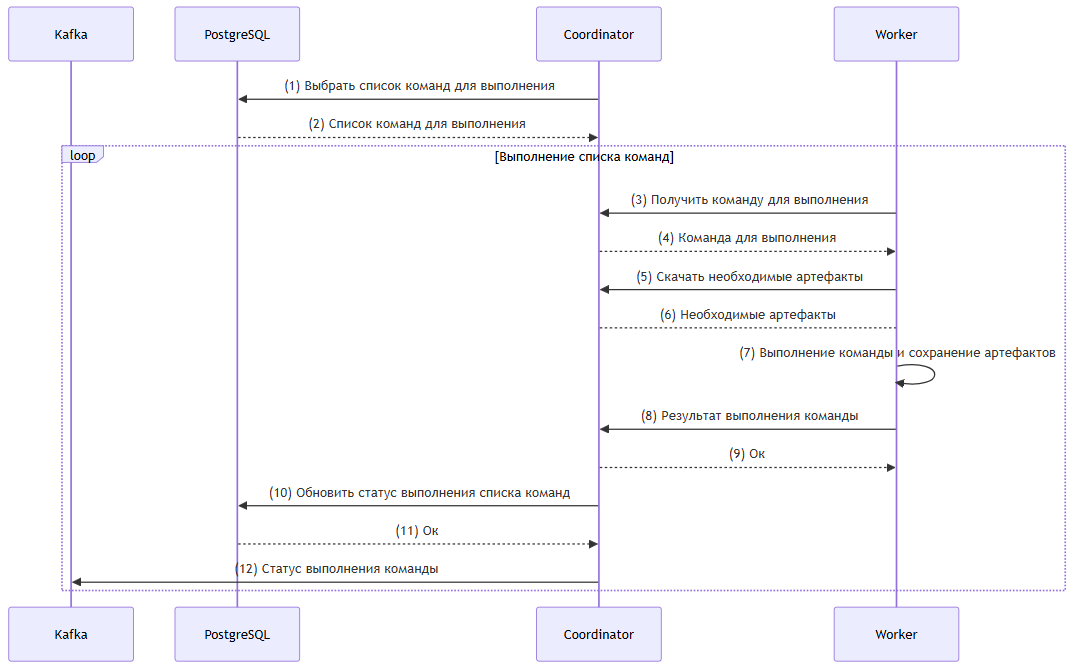
\includegraphics{images/execution-pipeline.png}
}
\caption{
\label{execution-pipeline}
     Процесс выполнения команд тестирования решений.}
\end{center}
\end{figure}

Coordinator выбирает очередной список команд для выполнения из PostgreSQL (1, 2).
Worker с заданным интервалом делает heartbeat-запрос (3) и получает команду для выполнения (4).
Для выполнения команды Worker скачивает необходимые артефакты (5, 6).
После выполнения команды Worker выполняет сохранение артефактов (7).
С результатом выполнения команды (8) Worker идёт в Coordinator (9).
Coordinator обновляет статус выполнения списка команд (10, 11) и отправляет статус выполнения команды в Kafka (12).

\subsubsection*{Анализ подозрительности поведения пользователя}

Для анализа подозрительности поведения Frontend собирает список действий пользователя в интерфейсе.
Analyzer по списку действий пользователя выдаёт степень подозрительности его поведения.
Процесс представлен на рисунке \ref{analyze-pipeline}.

\begin{figure}[ht]
\begin{center}
\scalebox{0.7}{
   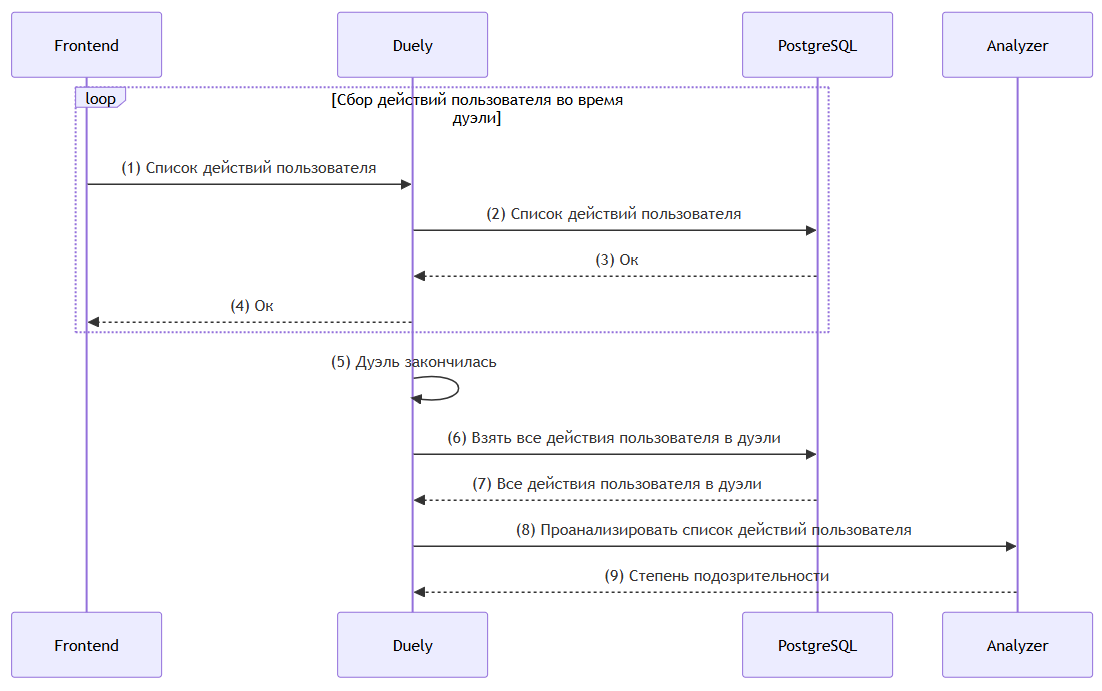
\includegraphics{images/analyze-pipeline.png}
}
\caption{
\label{analyze-pipeline}
     Процесс анализа поведения пользователя.}
\end{center}
\end{figure}

Во время дуэли Frontend собирает список действий пользователя и с заданным интервалом передаёт его в Duely (1, 4).
Duely сохраняет их в PostgreSQL (2, 3).
После окончания дуэли (5) Duely берёт все сохранённые действия пользователя в дуэли из PostgreSQL (6, 7).
Для анализа списка действий пользователя Duely делает запрос в Analyzer (8) и в ответе получает степень подозрительности (9).


\section{Распределённое тестирование решений}

Автоматическое тестирование представляет собой запуск решения на заранее подготовленных тестах и проверку ответа на каждом тесте.
Решение пользователя может быть написано на одном из разрешённых языков программирования (Python, C++, Go).
Некоторые из языков подразумевают предварительную компиляцию кода и запуск двоичного кода.
Проверка ответа выполняется с помощью чекера --- специальной программы,
которая также может быть реализована на одном из разрешённых языков программирования.

Процесс тестирования решения может быть представлен в виде ориентированного ацикличного графа,
вершинами которого являются атомарные команды (например, компиляция кода или запуск кода на одном тесте),
а ребро проводится из вершины A в вершину B, если выполнение команды B требует артефакты выполнения команды A.

Exesh предоставляет для использования несколько типов Job (команд):
\begin{itemize}
\item компиляция C++ кода;
\item компиляция Go кода;
\item запуск бинарного файла;
\item запуск Python кода;
\item запуск бинарного файла чекера.
\end{itemize}

На основе метаданных задачи и языка программирования решения компонент Taski формирует Execution ---
описание процесса тестирования в виде графа Jobs --- и отправляет его в Exesh для выполнения.
Добавление поддержки нового языка программирования требует лишь добавления нового типа Job в Exesh.
Добавление нового формата задачи требует добавления новой стратегии формирования Execution в Taski.
Далее процесс тестирования рассматривается как выполнение Execution, представляющего собой ориентированный ацикличный граф Jobs.

Так как не все Jobs в Execution зависят друг от друга последовательно, некоторые можно выполнять параллельно.
Пример параллельного исполнения графа Jobs показан на рисунке \ref{execution-graph}.
На нём разными цветами отмечены Jobs, которые могут быть выполнены на разных workers.
Такой подход позволяет эффективно использовать вычислительные ресурсы и сокращать суммарное время тестирования решений.

\begin{figure}[ht]
\begin{center}
\scalebox{0.6}{
   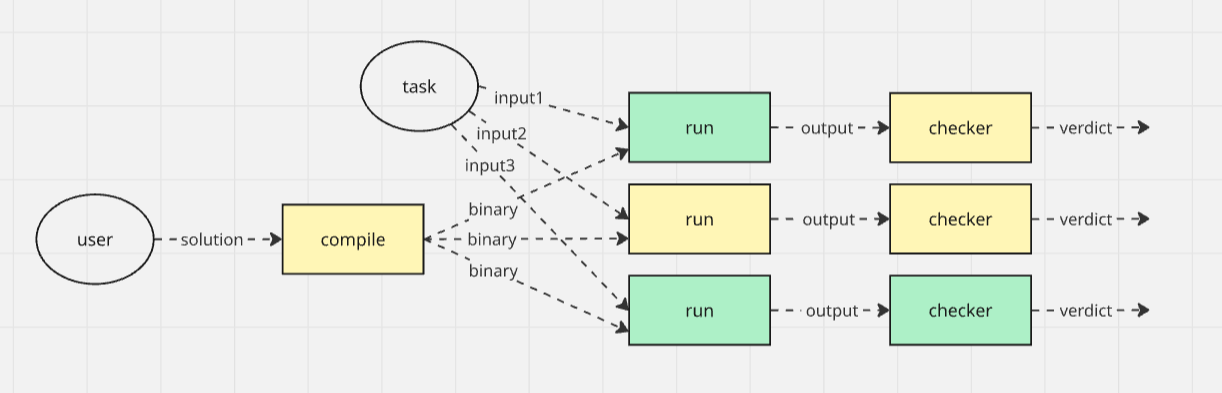
\includegraphics{images/execution-graph.png}
}
\caption{
\label{execution-graph}
     Пример распределённого исполнения Execution.}
\end{center}
\end{figure}

\subsection{Распределение ресурсов для исполнения набора Execution}

Пусть в момент времени $t$ система исполняет набор из $N$ Executions.
Пусть каждый Execution содержит $K_i$ Jobs ($i = 1, 2, \dots, N$).
Пусть каждый Job имеет ожидаемое время выполнения $time_{i, j}$ ($i = 1, 2, \dots, N$, $j = 1, 2, \dots, K_i$).
Оценка ожидаемого времени выполнения Job осуществляется при помощи статистических данных.
Используется предположение, что пользовательские решения на конкретном тесте в конкретной задаче имеют близкое время выполнения.

При последовательном выполнении всех Jobs в $i$-м Execution требуется $total_i = \sum_{j = 1}^{K_i} time_{i, j}$ времени.
Система имеет набор Workers, что позволяет исполнять Jobs параллельно и уменьшать реальное время исполнения Execution.
Пусть $i$-й Execution начал исполнение во время $start_i$.
Тогда в момент времени $t$ реальное время исполнения $i$-го Execution составляет $t - start_i$.

Задача заключается в выборе Execution, из которого должен быть выбран следующий Job для выполнения.
Иллюстрация задачи изображена на рисунке \ref{executions-problem}.

\begin{figure}[ht]
\begin{center}
\scalebox{0.4}{
   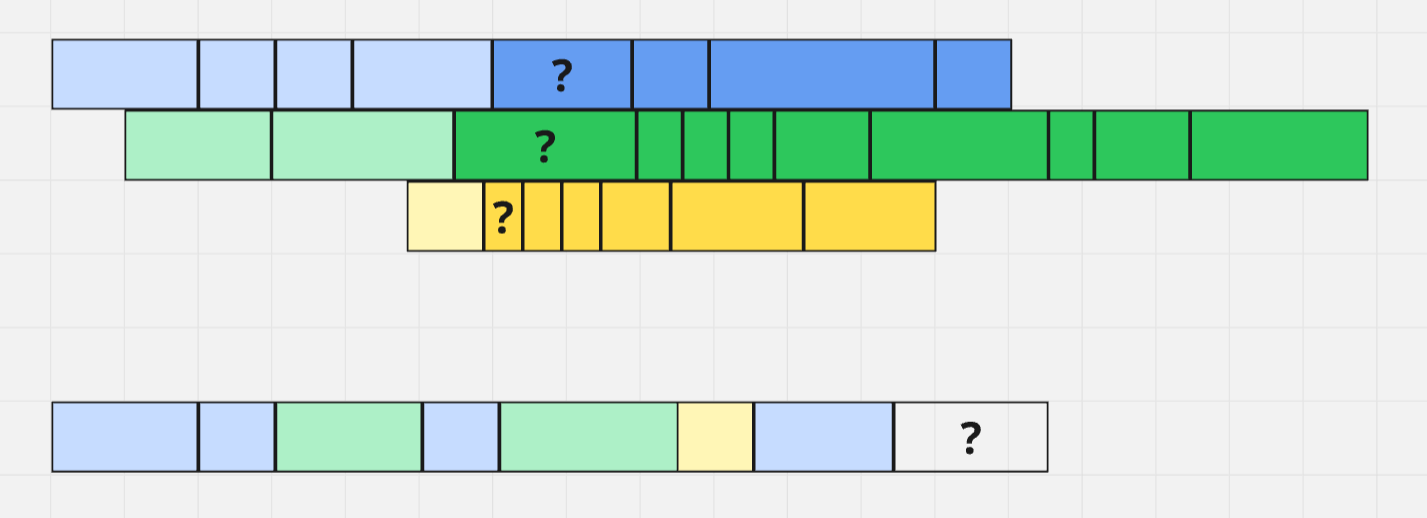
\includegraphics{images/executions-problem.png}
}
\caption{
\label{executions-problem}
     Задача выбора Execution для исполнения.}
\end{center}
\end{figure}

Введём функцию $priority(i, t)$ --- приоритет исполнения $i$-го Execution в момент времени $t$.
Подход заключается в сортировке Executions по их приоритету и выборе наиболее приоритетного Execution.

Рассмотрим, что должно влиять на приоритет Execution.
Во-первых, хочется, чтобы Execution, находящийся в системе дольше, получал больше ресурсов.
То есть приоритет должен зависеть от реального времени исполнения Execution.

Однако, если каждый раз выбирать самый старый живой Execution,
то получится так, что новые Executions не будут получать ресурсы, пока не закончат исполнение все ранее созданные.
Поэтому, во-вторых, на приоритет Execution должен влиять текущий прогресс исполнения.
Чем меньше ресурсов в относительном отношении получал Execution ранее, тем больше должен быть его приоритет.
Пусть в данный момент времени в $i$-м Execution были выполнены первые $F_i$ Jobs.
Прогресс должен быть рассчитан, исходя из ожидаемого времени выполнения Jobs,
поэтому для $i$-го Execution он будет равен $done_i = \sum_{j = 1}^{F_i} time_{i, j}$.

Также стоит сделать акцент на том, что разные Executions имеют разное суммарное ожидаемое время исполнения,
поэтому при подсчёте приоритета нужно использовать не абсолютное, а относительное время, зависящее от размера Execution.
Приоритет определяется следующим образом:

\begin{equation}
   priority(i, t) = \left(\frac{t - start_i}{total_i} + \alpha \cdot \frac{total_i - done_i}{total_i}\right) \times \gamma^{tries_i - 1}
\end{equation}

Формула содержит два основных компонента --- реальное время исполнения и ожидаемое время до конца исполнения.
Они по-разному должны влиять на приоритет, поэтому был введён параметр $\alpha$, определяющий отношение их влияния на приоритет.
Во время исполнения Execution может произойти ошибка (например, падение Coordinator).
В таком случае Execution будет перезапущен, но его приоритет при повторном запуске должен быть повышен.
Пусть $tries_i$ --- количество попыток выполнения $i$-го Execution,
тогда приоритет будет экспоненциально зависеть от этого значения и параметра $\gamma$.
Таким образом, приоритет увеличивается с ростом времени жизни Execution, при уменьшении доли уже выполненной работы,
а также при повторных запусках Execution после ошибок.

\subsection{Эффективное распределение Jobs по исполнителям}

Каждый worker в кластере имеет в своём распоряжении $S$ слотов.
Для выполнения одного Job требуется один слот на время выполнения Job.
Будем считать, что один слот соответствует $1$ CPU и $256$ MB RAM.
При этом Job может использовать больше $256$ MB RAM, но должно быть выполнено ограничение,
что в любой момент времени количество Jobs, выполняемых на worker, должно быть не более $S$,
а также что суммарный объём используемой памяти всеми выполняемыми Jobs должно не превышать $256 \cdot S$.

Пусть каждый Job имеет ожидаемый объём используемой памяти $memory_{i, j}$ ($i = 1, 2, \dots, N$, $j = 1, 2, \dots, K_i$).
Оценка ожидаемого объёма используемой памяти Job осуществляется при помощи статистических данных.
Используется предположение, что пользовательские решения на конкретном тесте в конкретной задаче имеют близкие значения памяти.

Каждый Job можно представить в виде прямоугольника с размерами $time \times memory$
на плоскости, в которой по оси Ox откладывается время, а по оси Oy --- память.
Для выполняемого Job ставится прямоугольник с левой стороной по координате начала выполнения,
и с правой стороной по ожидаемому окончанию выполнения.
В каждый момент времени любая прямая, параллельная оси Oy, должна пересекать не больше $S$ прямоугольников.

Рассмотрим очередной heartbeat-запрос от одного worker.
Нужно выбрать один Job, который отдать на выполнение этому worker.
Каждый worker имеет множество выполняемых в данный момент Jobs.
Имеется последовательность Executions, упорядоченная по приоритету, а каждый Execution предоставляет для выполнения один Job.

Простой алгоритм заключается в том, чтобы выбрать Job из самого приоритетного Execution и отдать его на выполнение.
Однако, такой алгоритм может неэффективно использовать ресурсы системы.
Пример проиллюстрирован на рисунке \ref{jobs-problem}.

\begin{figure}[ht]
\begin{center}
\scalebox{0.4}{
   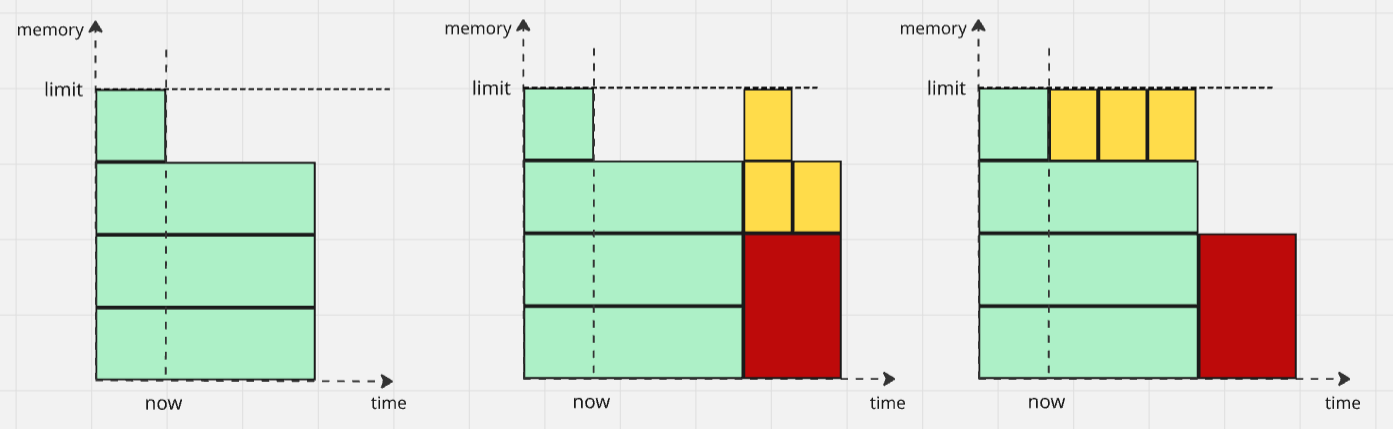
\includegraphics{images/jobs-problem.png}
}
\caption{
\label{jobs-problem}
     Задача распределения вычислительных ресурсов кластера.}
\end{center}
\end{figure}

Предположим, что в текущий момент времени есть большой более приоритетный Job (красного цвета)
и несколько маленьких менее приоритетных Jobs (жёлтого цвета).
Алгоритм, который всегда выбирает Job из наиболее приоритетного Execution,
в момент текущий момент времени не может отдать на выполнение красный Job, и ему приходится ждать окончания уже выполняемых Jobs.
Однако, эффективный способ утилизации ресурсов заключается в том,
что можно выполнить менее приоритетные жёлтые Jobs перед более приоритетным красным,
и этом ожидаемое время начала выполнения более приоритетного Job не изменится,
что позволяет повысить утилизацию ресурсов без ухудшения работы предыдущего алгоритма.

Псевдокод promise-based алгоритма выглядит следующим образом:

\begin{minted}{python}
def schedule(jobs, promised_jobs):
   for job in promised_jobs:
      if can_start_now(job):
         start(job)
         return
   
   jobs.sort(key=job.priority)

   for job in jobs:
      if can_start_now(job):
         start(job)
         return
      elif len(promised_jobs) < limit:
         start_time = get_start_time(job)
         promise(job, start_time)
\end{minted}

Суть алгоритма заключается в том, что он пытается понять, может ли запустить сейчас самый приоритетный Job,
и если может, то запускает, а если нет, то вычисляет минимальное возможное время начала и резервирует его.
Когда возникает очередная возможность запустить Job, алгоритм сначала пытается запустить promised Jobs,
а если не получается, то пытается запустить остальные в порядке приоритета.
Алгоритм использует две основные функции:
\begin{itemize}
\item can\_start\_now(job) --- можем ли сейчас запустить job, не нарушив существующие резервации;
\item get\_start\_time(job) --- минимальное время, в которое получится запустить job, не нарушив существующие резервации.
\end{itemize}

Алгоритм принимает решения, используя только текущую информацию о выполняемых Jobs и статистические оценки ресурсов,
поэтому вводится ограничение на максимальное количество promised Jobs,
чтобы не происходило деградации планировщика из-за большого количества зарезервированных Jobs.

\subsection{Исполнение команд в изолированном окружении}

Исполнение команд предполагает запуск произвольного пользовательского кода в системе.
Это может повлечь серьёзные последствия для инфраструктуры платформы, если не вводить ограничения на действия пользовательского кода.

При выполнении пользовательского кода необходимо ограничивать следующие возможности:
\begin{itemize}
\item доступ к файловой системе вне рабочей директории;
\item взаимодействие с сетевым интерфейсом;
\item создание новых процессов и потоков;
\item превышение использования процессорного времени и оперативной памяти;
\item выполнение потенциально опасных системных вызовов.
\end{itemize}

Также необходимо ограничивать время выполнения и объём используемой памяти.
Измерение должно производиться по времени исполнения процесса на процессоре, а не по реальному времени,
что позволяет избежать ошибок, вызванных конкурентным выполнением других процессов,
и обеспечить повторяемость результатов независимо от текущей нагрузки системы.

Для запуска пользовательского кода была выбрана утилита isolate,
которая разработана специально для использования в системах автоматического тестирования решений.
Утилита использует механизмы изоляции процессов Linux, такие как namespaces и cgroups,
что позволяет ограничивать доступ программы к системным ресурсам и изолировать процессы друг от друга.

Выбор isolate вместо разработки собственной системы изоляции процессов был обусловлен
её широким использованием в системах автоматического тестирования решений (например, на IOI),
что является хорошим подтверждением надёжности утилиты, а также низкими накладными затратами на использование.
По сравнению с реализацией на основе Docker-контейнеров, isolate позволяет уменьшить время запуска команд,
что особенно важно при большом количестве короткоживущих процессов тестирования.

\subsection{Подход к взаимодействию с файловой системой}

Для взаимодействия с файловой системой в компонентах Taski и Exesh используется библиотека filestorage,
которая была написана специально для этого проекта и поддерживает эффективный и конкурентный доступ к ресурсам системы.

Библиотека оперирует понятием бакет --- независимая единица разделения файловой системы.
Бакет является папкой, которая может содержать другие папки и файлы, но не бакеты.
Каждый бакет имеет уникальный идентификатор, представляющий собой SHA-1 хеш длиной 20 байт (40 hex-символов).
Бакеты разделяются на 256 шардов (по первым двум hex-символам идентификатора), каждый из которых лежит в отдельной папке.
Такое разделение уменьшает количество объектов внутри одной директории и повышает эффективность работы с файловой системой.
Каждый бакет имеет время жизни либо является бессрочным.
Библиотека поддерживает автоматическое удаление бакетов по истечении их времени жизни.

Библиотека позволяет передавать бакеты и отдельные файлы между компонентами системы.
Передача ресурсов осуществляется в формате tar-stream с использованием сжатия.
Ресурсы сначала скачиваются во временную папку, а затем переносятся в основное хранилище.
Интерфейс библиотеки предоставляет методы commit и abort, которые влияют на перенос ресурсов в основное хранилище из временного.
Если бакет или файл уже присутствует в локальном хранилище, повторная загрузка не выполняется.

\subsection{Нагрузочное тестирование системы}

Для нагрузочного тестирования был использован сервер с конфигурацией $8$ CPU с тактовой частотой $3.3$ ГГц и $8$ ГБ RAM.
На сервере были развёрнуты компоненты Duely, Analyzer, Taski, Exesh и Dashboard.
В Exesh был кластер с двумя workers и одним coordinator.
Каждый worker имеет возможность одновременно исполнять $4$ Jobs, то есть всего одновременно может исполняться $8$ Jobs.

Предполагалось, что компонентами системы суммарно будет использоваться $1$ CPU,
а остальные $7$ CPU будет выделено планировщиком операционной системы для запуска пользовательского кода.
Производился запуск трёх наборов по пять Executions, между которыми был отступ $5$ секунд.
Между Executions в одном наборе был случайный отступ от $1$ до $3$ секунд.
Все Executions содержали по $50$ Jobs, каждый из которых выполняется $1$ секунду.

Если производить последовательный запуск всех Jobs на одном CPU, то потребуется $1 \cdot 50 \cdot 15 = 750$ секунд.
В результате нагрузочного тестирования было определено,
что между началом первого Execution и окончанием последнего проходит $105$ секунд.
Таким образом, параллельная обработка на $8$ CPU происходит в $7.14$ раз быстрее, чем последовательная на одном CPU.
Результат оказался вполне достойным --- компонентами системы суммарно использовалось даже меньше $1$ CPU,
а все остальные ресурсы были выделены для запуска пользовательского кода.
В то же время, при увеличении количества CPU выделение ресурсов для компонентов системы растёт не так быстро,
и эффективность параллельного исполнения приближается к количеству CPU.

Также проводилось тестирование разных алгоритмов подсчёта приоритета Execution.
Были рассмотрены формулы, которые учитывают только реальное время исполнения, только ожидаемое оставшееся время исполнения,
а также учитывающие оба фактора, но с разными значениями коэффициента $\alpha$.
Для сравнения были выбраны графики, иллюстрирующие изменение приоритета и прогресса Execution.

Графики, получившиеся при расчёте приоритета, исходя только из реального времени исполнения ($\alpha = 0$),
изображены на рисунках \ref{priority_alpha-0} и \ref{progress_alpha-0}.
Видно, что приоритеты растут линейно и следующий Execution не начинают исполнение до окончания предыдущего.

\begin{figure}[ht]
\begin{center}
\scalebox{0.3}{
   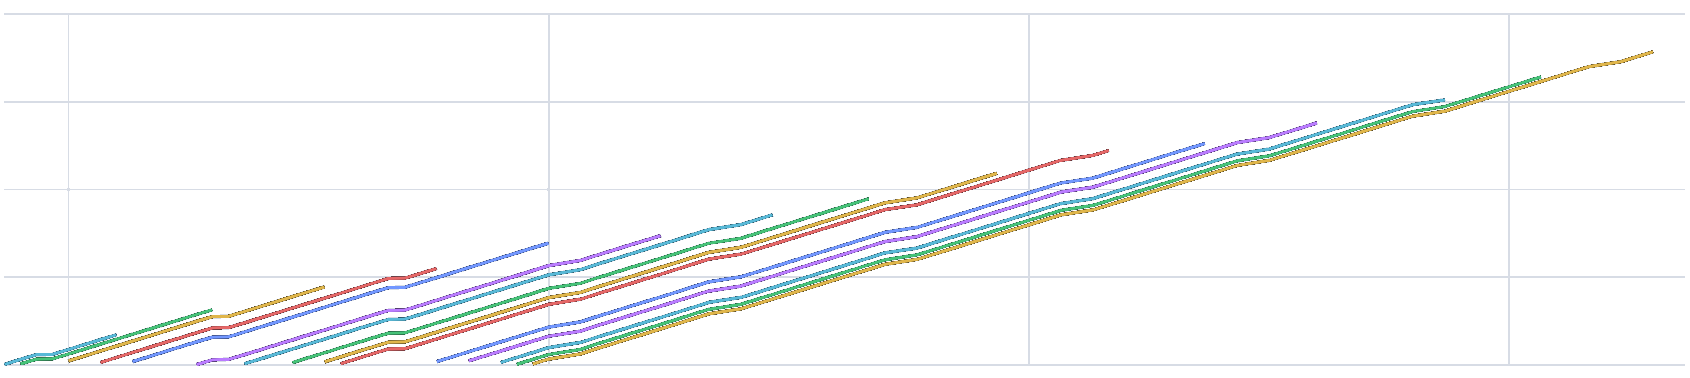
\includegraphics{images/executions/priority_alpha-0.png}
}
\caption{
\label{priority_alpha-0}
     Изменение приоритетов при $\alpha = 0$.}
\end{center}
\end{figure}

\begin{figure}[ht]
\begin{center}
\scalebox{0.3}{
   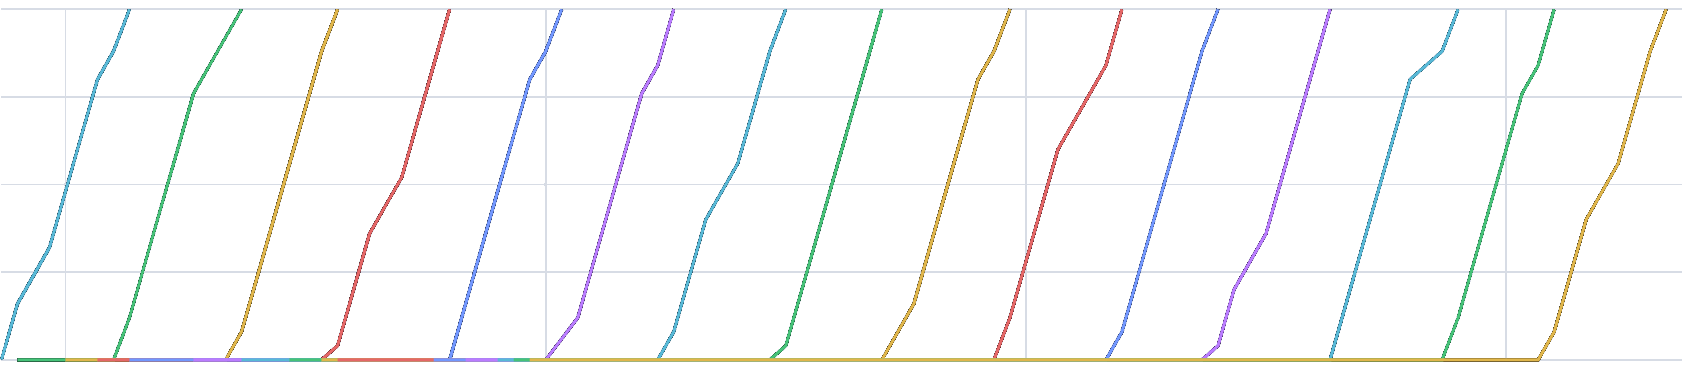
\includegraphics{images/executions/progress_alpha-0.png}
}
\caption{
\label{progress_alpha-0}
     Изменение прогрессов при $\alpha = 0$.}
\end{center}
\end{figure}

Графики, получившиеся при расчёте приоритета, исходя только из ожидаемого оставшегося времени исполнения ($\alpha \to \infty$),
изображены на рисунках \ref{priority_alpha-inf} и \ref{progress_alpha-inf}.
Видно, что приоритеты уменьшаются с течением времени, а также что в какой-то момент все приоритеты выравниваются,
и остаются таковыми до конца исполнения всех Executions, которые заканчивают исполнение одновременно.

\begin{figure}[ht]
\begin{center}
\scalebox{0.3}{
   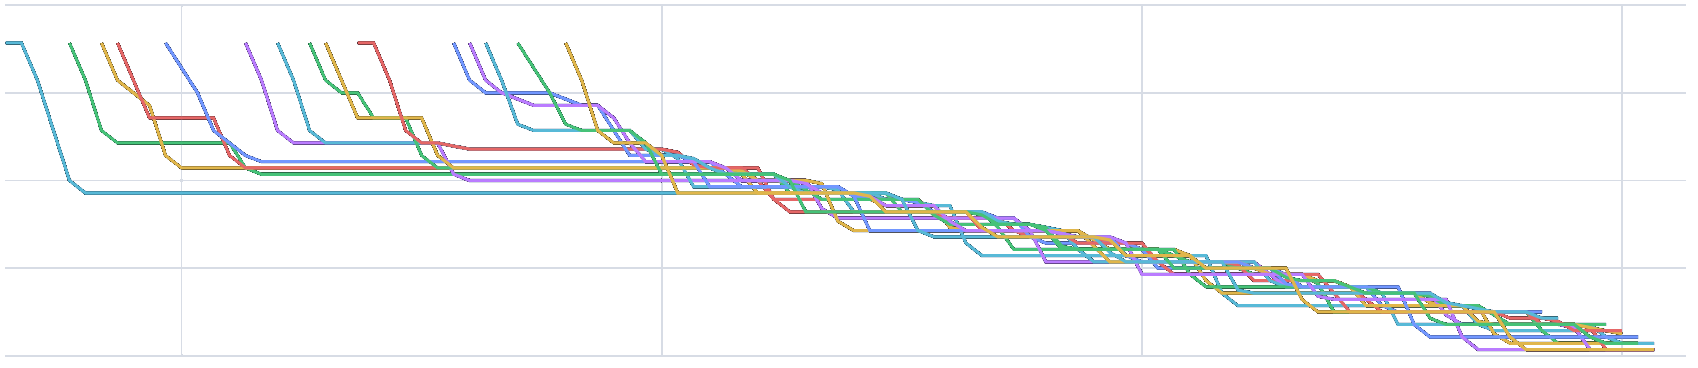
\includegraphics{images/executions/priority_alpha-inf.png}
}
\caption{
\label{priority_alpha-inf}
     Изменение приоритетов при $\alpha \to \infty$.}
\end{center}
\end{figure}

\begin{figure}[ht]
\begin{center}
\scalebox{0.3}{
   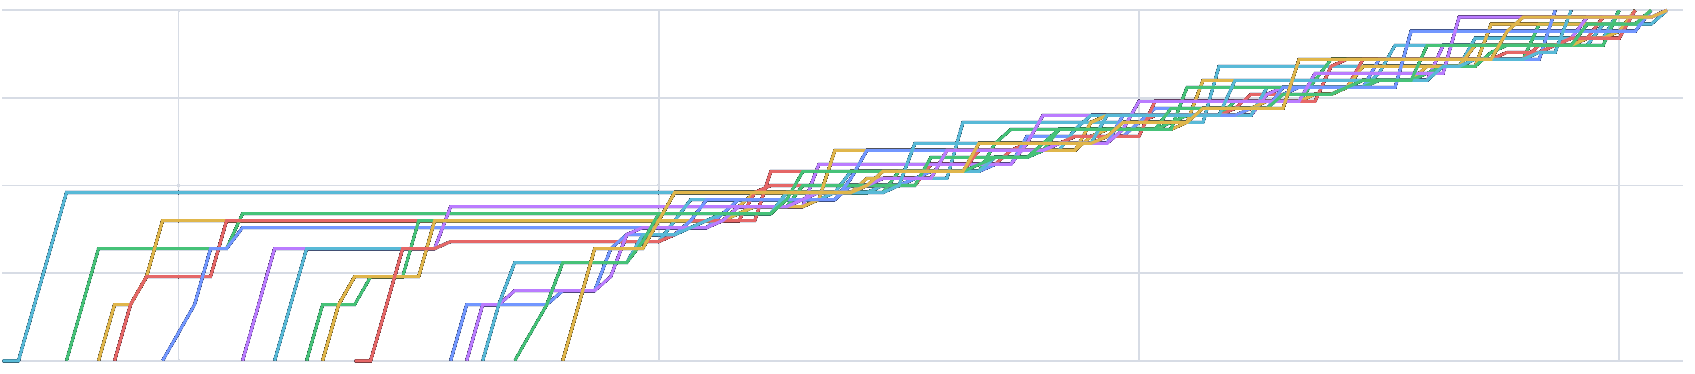
\includegraphics{images/executions/progress_alpha-inf.png}
}
\caption{
\label{progress_alpha-inf}
     Изменение прогрессов при $\alpha \to \infty$.}
\end{center}
\end{figure}

Графики, получившиеся при расчёте приоритета при учёте обоих факторов и значения $\alpha = 1$,
изображены на рисунках \ref{priority_alpha-1} и \ref{progress_alpha-1}.
Видно, что графики похожи на графики с $\alpha = 0$, но при этом можно наблюдать,
что изменения прогрессов происходят не линейно, а постепенно ступеньками,
и это означает, что планировщик чаще переключается между различными Executions, чем заканчивает исполнение очередного Execution.

\begin{figure}[ht]
\begin{center}
\scalebox{0.3}{
   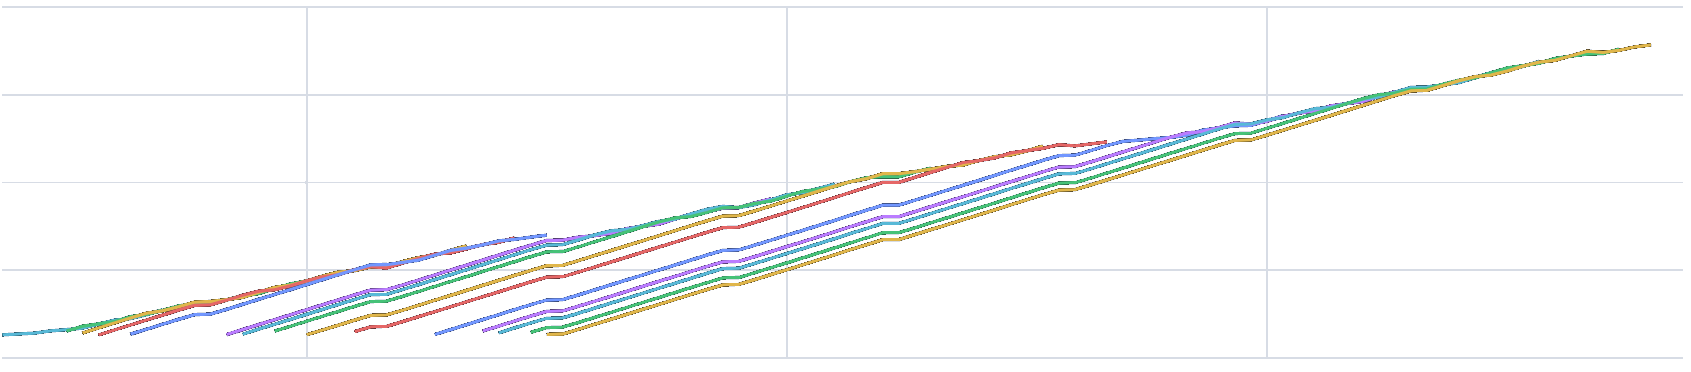
\includegraphics{images/executions/priority_alpha-1.png}
}
\caption{
\label{priority_alpha-1}
     Изменение приоритетов при $\alpha = 1$.}
\end{center}
\end{figure}

\begin{figure}[ht]
\begin{center}
\scalebox{0.3}{
   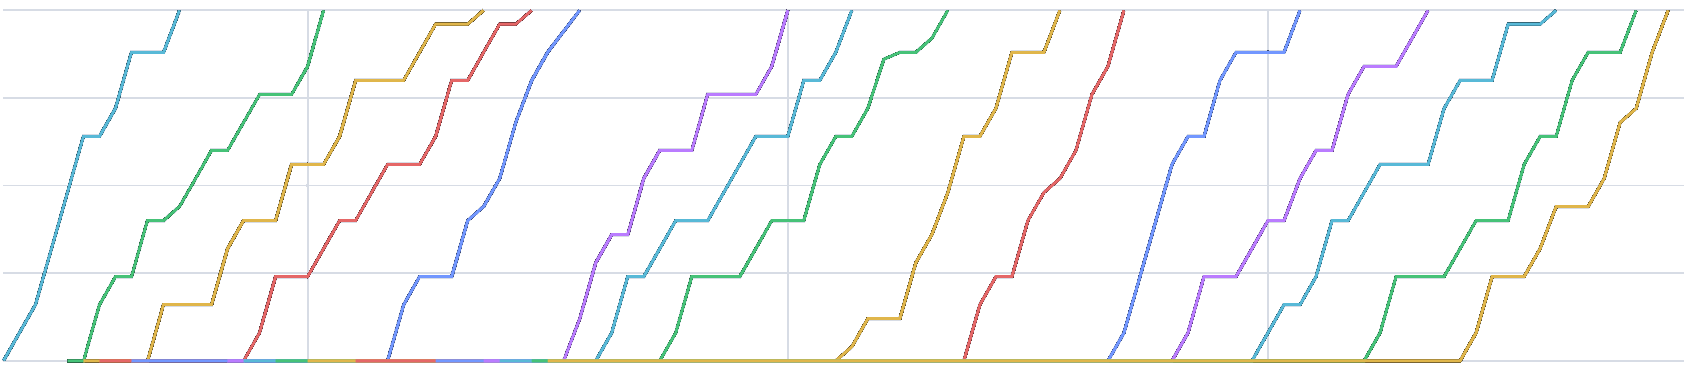
\includegraphics{images/executions/progress_alpha-1.png}
}
\caption{
\label{progress_alpha-1}
     Изменение прогрессов при $\alpha = 1$.}
\end{center}
\end{figure}

Графики, получившиеся при расчёте приоритета при учёте обоих факторов и значения $\alpha = 10$,
изображены на рисунках \ref{priority_alpha-10} и \ref{progress_alpha-10}.
Видно, что выбор Execution меняются достаточно часто, но реже, чем при $\alpha = \inf$,
и ранее появившийся Execution получает допустимое преимущество относительно более поздних Executions.

\begin{figure}[ht]
\begin{center}
\scalebox{0.3}{
   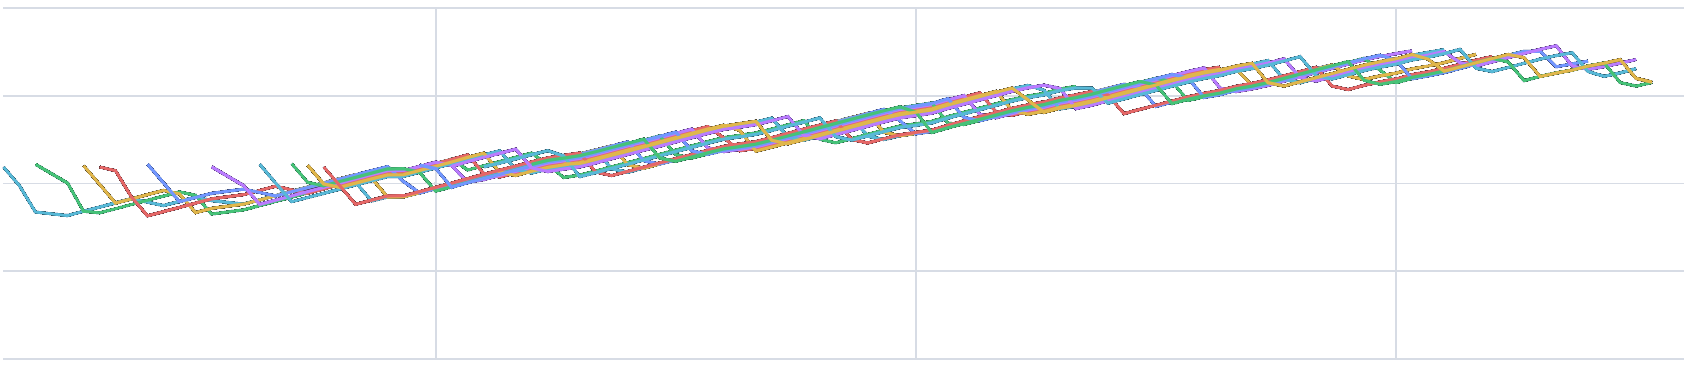
\includegraphics{images/executions/priority_alpha-10.png}
}
\caption{
\label{priority_alpha-10}
     Изменение приоритетов при $\alpha = 10$.}
\end{center}
\end{figure}

\begin{figure}[ht]
\begin{center}
\scalebox{0.3}{
   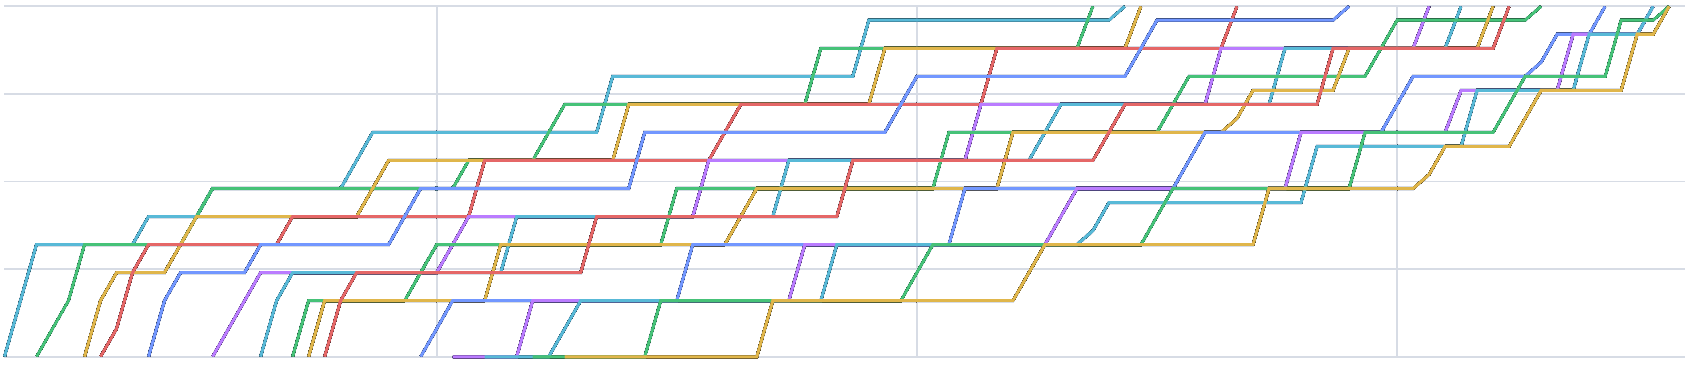
\includegraphics{images/executions/progress_alpha-10.png}
}
\caption{
\label{progress_alpha-10}
     Изменение прогрессов при $\alpha = 10$.}
\end{center}
\end{figure}

\subsubsection*{Выводы}

В ходе нагрузочного тестирования было показано,
что предложенный подход к распределению ресурсов позволяет эффективно использовать вычислительные ресурсы системы
и обеспечивает высокую степень параллельности исполнения.
Также было определено, что использование только время существования Execution приводит к эффекту застоя для новых Executions,
в то время как использование только ожидаемого оставшегося времени приводит к чрезмерно равномерному распределению ресурсов.
Наиболее сбалансированное поведение системы наблюдается при использовании комбинированной формулы приоритета,
учитывающей как время существования Execution, так и ожидаемое оставшееся время выполнения.


\section{Анализ подозрительности пользователя}

\subsection{Постановка задачи}

Поведение пользователя во время решения задачи представляет собой последовательность
действий написания кода и взаимодействия с тестирующей системой.
Нечестное участие в дуэли подразумевает собой использование сторонних инструментов, помогающих в решении задачи.
В роли таких инструментов могут выступать модели искусственного интеллекта для генерации кода.
Также нечестным поведением является поиск готового кода в интернете и его использование для решения задачи.

Характер написания кода при использовании сторонних инструментов отличается от обычного процесса разработки решения.
Задача состоит в определении поведенческих паттернов человека во время решения задачи и
разработке системы, вычисляющей степень подозрительности поведения пользователя.

Стоит отметить, что задача не предполагает точного доказательства факта нечестного поведения.
Система будет лишь оценивать степень отклонения поведения пользователя от обычного процесса разработки решения и
может быть использована в качестве инструмента для выявления подозрительных пользователей, требующих дополнительной проверки.

Формально, есть последовательность событий $E = \{e_1, e_2, \dots, e_n\}$, где $e_i$ --- событие с временной меткой и типом.
Требуется построить отображение $f(E) \to p \in [0, 1]$,
где $p$ --- степень подозрительности поведения пользователя ($p = 0$ --- поведение нормальное, $p = 1$ --- поведение подозрительное).

\subsection{Анализ поведенческих паттернов}

Во время честного решения задачи количество строк кода растёт нелинейно относительно времени,
изменения достаточно неоднородны, иногда происходит возврат к ранее написанным строкам или просто прыжок в другую часть кода.
Также достаточно часто человек может использовать свои личные заготовки кода и вставлять их в редактор,
однако после этого непременно происходит редактирование вставленной части кода.
Процесс решения задачи можно разбить на этапы продумывания и написания кода.
Причём количество этапов продумывания кода обычно зависит от сложности задачи и количества строк в решении.
Можно рассмотреть среднюю скорость добавления символов в этапы написания кода,
но она достаточно сильно зависит от человека и не может служить признаком подозрительности поведения.
Однако, скорость написания кода достаточно редко бывает постоянной,
поэтому в качестве признака можно будет взять среднее отклонение средней скорости написания кода.
Также характерным признаком разработки решения задачи являются этапы отладки кода,
которые представляют собой тестирование решения, перемещение курсора по коду, внесение небольших изменений.

Стоит также рассмотреть сценарии нечестного написания кода при помощи вспомогательных инструментов.
Большинство подобных сценариев может быть выявлено по вставке большого объёма кода без последующего изменения.
Если человек более осторожен, он может вставлять код кусками, однако также без изменений вставленных участков кода.
Ещё одним сценарием также является ручное перепечатывание кода из другого места.
В таком случае будет мало перемещений между разными участками кода и исправлений уже написанных строк.
При использовании генеративных моделей, которые самостоятельно пишут код в редактор кода, можно заметить,
что скорость добавления нового кода достаточно постоянна и редко отклоняется от среднего значения,
а также код растёт линейно и отсутствуют перемещения курсора.

\subsection{Сбор и преобразование данных}

Так как пользователь во время участия в дуэли пишет код в браузере,
есть возможность собирать события из редактора кода: изменение, вставка, удаление кода и перемещение курсора.
Также будут собираться события взаимодействия с системой: выбор языка программирования, запуск теста и отправка на проверку.

Эти события будут собираться на фронтенде и с некоторым интервалом отправляться на бэкенд.
Бэкенд будет сохранять их в базе данных для последующего анализа.
После окончания дуэли можно будет проанализировать поведение каждого пользователя при решении задачи.

Последовательность событий $E$ будет преобразована к виду, который будет удобен для работы $t(E) \to x \in \mathbb{R}^d$.
Другими словами, последовательность событий будет преобразована к табличному виду, будет произведено выделение признаков.

Для анализа был выделен следующий набор признаков:
\begin{itemize}
\item $typing\_speed\_avg$ --- средняя скорость ввода кода;
\item $typing\_speed\_std$ --- разброс скорости ввода кода;
\item $typing\_intervals\_count$ --- количество этапов ввода кода;
\item $typing\_interval\_duration\_avg$ --- среднее время этапа ввода кода;
\item $edits\_count$ --- общее количество изменений кода;
\item $edit\_size\_avg$ --- средний размер одного изменения кода;
\item $edit\_size\_max$ --- максимальный размер одного изменения кода;
\item $edit\_size\_std$ --- разброс размеров изменений кода;
\item $small\_edits\_ratio$ --- доля мелких изменений кода;
\item $paste\_count$ --- количество вставок кода;
\item $paste\_size\_avg$ --- средний размер вставки кода;
\item $paste\_size\_max$ --- максимальный размер вставки кода;
\item $paste\_edited\_ratio$ --- доля событий изменения после вставки кода;
\item $cursor\_jump\_count$ --- количество перемещений в другую часть кода;
\item $run\_test\_count$ --- количество запусков кода на тестах;
\item $submit\_count$ --- количество отправок на проверку;
\item $user\_rating$ --- рейтинг пользователя.
\end{itemize}

\subsection{Моделирование подозрительности}

Задача моделирования подозрительности формулируется как задача бинарной классификации:
по набору признаков требуется оценить вероятность принадлежности поведения пользователя к подозрительному классу.
Полученное значение интерпретируется как степень подозрительности.

В качестве моделей были выбраны логистическая регрессия и метод случайного леса.
Логистическая регрессия имеет высокую интерпретируемость и малый риск переобучения.
Она позволит получить достаточно стабильную базовую оценку.
Метод случайного леса способен учитывать сложные нелинейные зависимости между признаками,
которые характерны для поведенческих данных пользователей.
Использование более сложных моделей, например, нейронных сетей, будет избыточным.

\subsection{Сбор и разметка обучающих данных}

Анализ поведения пользователя во время написания кода не является хорошо изученной задачей,
поэтому не удалось найти датасеты для обучения моделей в открытых источниках.
Исходя из этого, обучающие данные были собраны следующими подходами:
\begin{itemize}
\item самостоятельное участие в дуэлях и решение задач как честно, так и с использованием сторонних инструментов;
\item проведение турнира на кружке по олимпиадному программированию СПбГУ;
\item генерация синтетических последовательностей событий, имитирующих различные стратегии поведения пользователя.
\end{itemize}

\subsection{Качество работы моделей}

Метрики качества работы моделей представлены на рисунке \ref{analyzer-metrics}.
Несмотря на маленький объём обучающей и тестовой выборок, обе модели показали достаточно хорошие результаты.

Значение метрики $recall$, близкое к $1$, означает, что модели очень редко пропускают действительно нечестных пользователей.
При этом имеется достаточно высокое значение $false\_positive\_rate$ (порядка $0.2$),
однако это лишь значит, что модели слишком подозрительны к поведению и чаще нужного подозревают честных пользователей.
Если повышать $threshold$, после которого считать пользователя подозрительным,
то $false\_positive\_rate$ закономерно уменьшается, но страдает $recall$.
Для системы оценки подозрительности пользователей лучше иметь слегка завышенный $false\_positive\_rate$, чем заниженный $recall$,
чтобы реже пропускать действительно нечестных пользователей.

По валидационным графикам, а также по roc-кривой можно увидеть, что
модель логистической регрессии в среднем имеет более хорошие значения метрик,
нежели модель с использованием метода случайного леса.
Это можно объяснить тем, что собранная обучающая выборка имеет довольно маленький объём,
и случайный лес достигает большей перетренированности, чем логистическая регрессия.

\begin{figure}[ht]
\begin{center}
\scalebox{0.4}{
   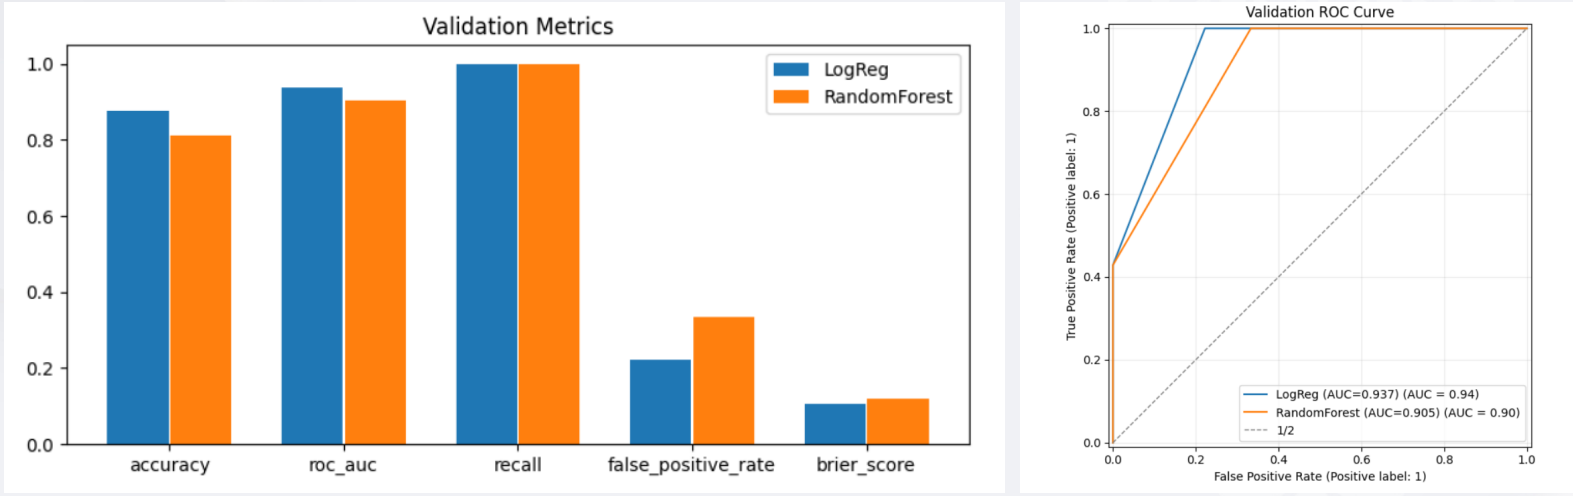
\includegraphics{images/analyzer-metrics.png}
}
\caption{
\label{analyzer-metrics}
     Метрики качества работы моделей.}
\end{center}
\end{figure}

\specialsection{Заключение}

В рамках выпускной квалификационной работы был разработан комплекс информационных систем
для проведения соревнований и тренировок по спортивному программированию в формате дуэлей.
Разработанная система поддерживает проведение рейтинговых и дружеских дуэлей, управление группами пользователей,
организацию турниров, автоматическое тестирование решений, а также анализ поведения участников во время решения задач.

Пользовательский Web-интерфейс позволяет пользователям входить в систему,
участвовать в дуэлях, использовать функционал групп и турниров.
Пример интерфейса участия в дуэли представлен на рисунке \ref{duel-interface}.
На экране дуэли отображаются редактор кода, условие задачи, доступные тесты и элементы управления запуском решения.

\begin{figure}[ht]
\begin{center}
\scalebox{0.3}{
   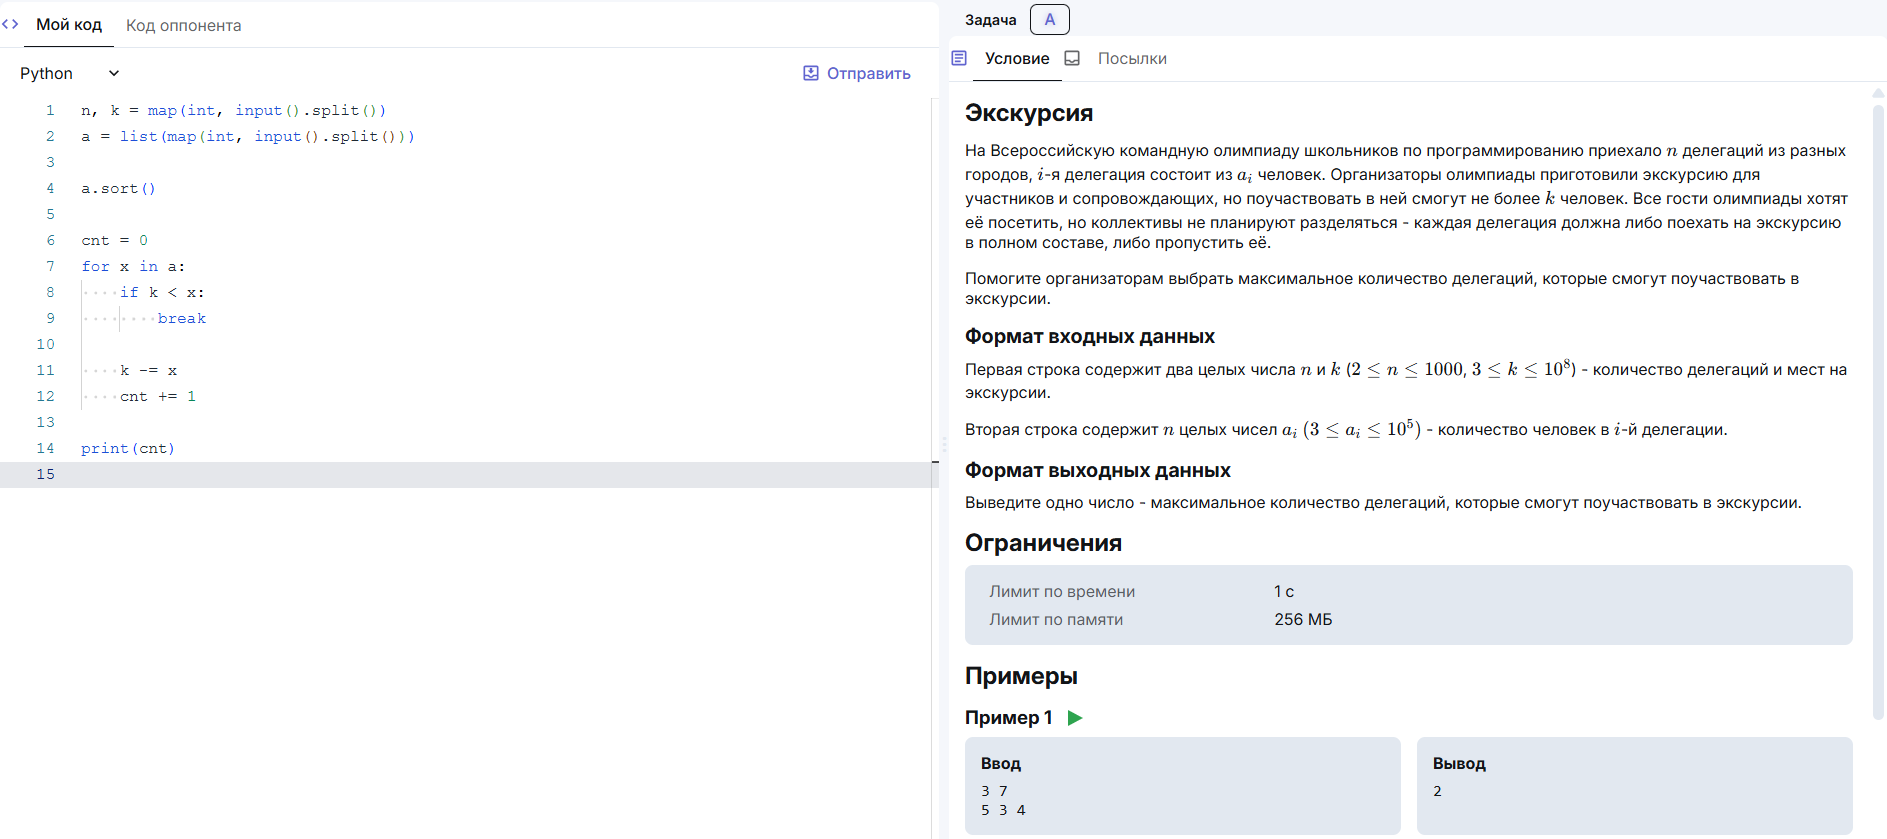
\includegraphics{images/duel-interface.png}
}
\caption{
\label{duel-interface}
     Интерфейс участия в дуэли.}
\end{center}
\end{figure}

Также в качестве примера интерфейса на рисунке \ref{tournament-interface} показан экран с результатами турнира, проведенного в СПбГУ.
На интерфейсе отображается турнирная таблица, а также результаты дуэлей между участниками турнира.

\begin{figure}[ht]
\begin{center}
\scalebox{0.6}{
   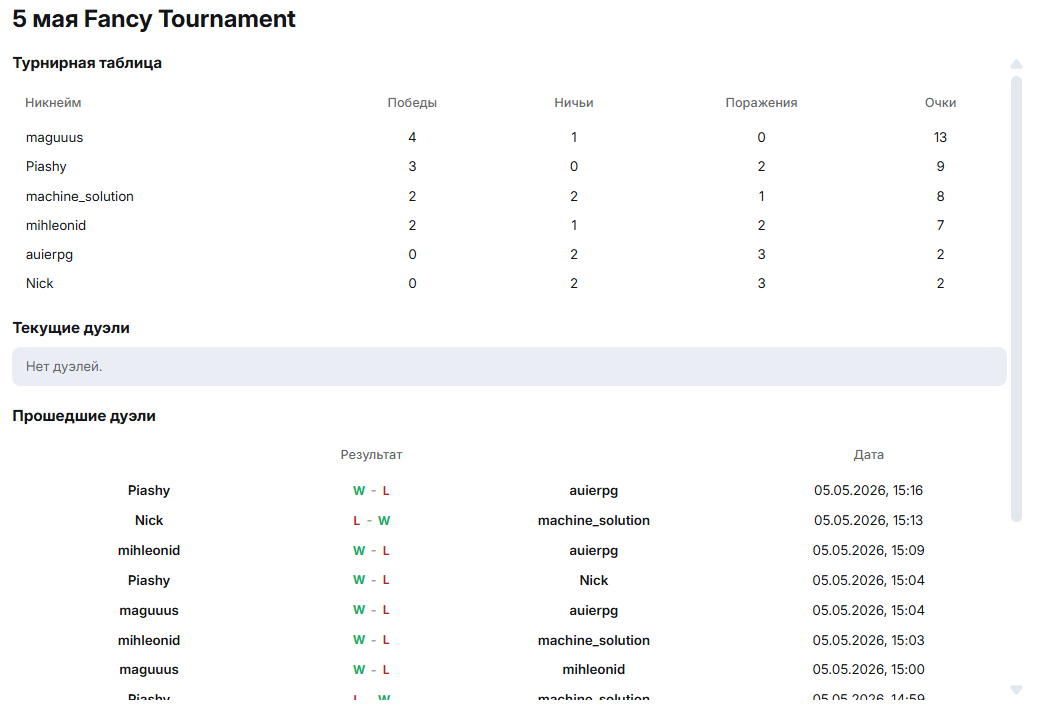
\includegraphics{images/tournament-interface.png}
}
\caption{
\label{tournament-interface}
     Интерфейс турнира.}
\end{center}
\end{figure}

Была спроектирована распределённая микросервисная архитектура системы,
включающая компоненты Frontend, Duely, Taski, Exesh, Analyzer и Dashboard.
Для взаимодействия компонентов использовались HTTP, WebSocket и Kafka.
Разработанная архитектура позволяет масштабировать систему и эффективно распределять вычислительные ресурсы между компонентами.

Автоматическое тестирование решения было рассмотрено в виде ориентированного ацикличного графа Jobs.
Для распределения вычислительных ресурсов был разработан алгоритм планирования Executions,
учитывающий как время существования Execution, так и прогресс его выполнения.
Также был предложен алгоритм распределения Jobs по Workers, позволяющий повысить эффективность использования ресурсов системы.
Проведённое нагрузочное тестирование показало, что система эффективно использует вычислительные ресурсы
и обеспечивает высокую степень параллельности выполнения задач.

Для исполнения пользовательского кода был реализован запуск команд в изолированном окружении с использованием утилиты isolate.
Дополнительно была разработана библиотека filestorage, обеспечивающая хранение и передачу файлов между компонентами системы.

Отдельное внимание в работе было уделено анализу поведения пользователей во время решения задач.
Была поставлена задача оценки степени подозрительности поведения пользователя, сформирован набор поведенческих признаков,
а также реализованы модели машинного обучения.
Полученные результаты показали, что предложенный подход позволяет выявлять отклонения от обычного процесса разработки решения
и может использоваться как вспомогательный инструмент для обнаружения нечестных пользователей, использующих сторонние инструменты.

Разработанная система может быть использована как платформа для проведения дуэлей по спортивному программированию,
а также как основа для дальнейших исследований в области распределённого тестирования решений и анализа поведения пользователей.
В дальнейшем возможным направлением развития является развитие моделей анализа поведения пользователей,
добавление в систему новых и разнообразных типов задач и увеличение набора функциональных требований.




% Аргумент {1} ниже включает переопределенный стиль с выравниванием слева
\begin{thebibliography}{1}
    \bibitem{pinedo} Scheduling Theory, Algorithms and Systems (Pinedo, 2008).
    \bibitem{queueing} Performance Modeling and Design of Computer Systems. Queueing Theory in Action.
    \bibitem{srpt} On the SRPT Scheduling Discipline in Many-Server Queues with Impatient Customers \url{https://arxiv.org/abs/2102.05789}.
    \bibitem{wfq} Алгоритмы Weighted fair queueing \url{https://en.wikipedia.org/wiki/Weighted_fair_queueing}.
    \bibitem{doc-isolate} Документация утилиты isolate \url{https://www.ucw.cz/isolate/isolate.1.html}.
    \bibitem{git-isolate} Репозиторий утилиты isolate \url{https://github.com/ioi/isolate}.
    \bibitem{distbuild} Сборка и тестирование в монорепозитории: кластер распределённой сборки DistBuild \url{https://habr.com/ru/companies/yandex/articles/565568/}.
    \bibitem{react} React документация \url{https://react.dev/}.
    \bibitem{logreg-scikit} Документация по Логистической регрессии от scikit-learn \url{https://scikit-learn.org/stable/modules/generated/sklearn.linear_model.LogisticRegression.html}.
    \bibitem{random-forest} Random Forest: прогулки по зимнему лесу \url{https://habr.com/ru/articles/320726/}.
    \bibitem{random-scikit} Документация по Random Forest от scikit-learn \url{https://scikit-learn.org/stable/modules/generated/sklearn.ensemble.RandomForestClassifier.html}.
    \bibitem{sklearn} Scikit-learn: Machine Learning in Python (Fabian Pedregosa, 2011) \url{https://jmlr.org/papers/volume12/pedregosa11a/pedregosa11a.pdf}.
\end{thebibliography}
\end{document}
